% ================= IF YOU HAVE QUESTIONS =======================
% Technical questions to bbob@lri.fr
% ===============================================================
%
\documentclass{article}
%%%%%%%%%%%%%%%%%%%%%%%%%%%%    PREAMBLE   %%%%%%%%%%%%%%%%%%%%%%%%%%%%%%%%%%%%
\usepackage{graphicx}
\usepackage[dvipsnames]{xcolor}
\usepackage{rotating}
\usepackage{amsmath}
\usepackage{caption,subfig}
\usepackage{xstring} % for string operations
\usepackage{wasysym} % Table legend with symbols input from post-processing
\usepackage{MnSymbol} % Table legend with symbols input from post-processing

\captionsetup[subfloat]{labelformat=empty,font=normalsize,position=top}
%%%%%%%%%%%%%%%%%%%%%%   END OF PREAMBLE   %%%%%%%%%%%%%%%%%%%%%%%%%%%%%%%%%%%%

%%%%%%%%%%%%%%%%%%%%%%%%%%%%%%%%%%%%%%%%%%%%%%%%%%%%%%%%%%%%%%%%%%%%%%%%%%%%%%%
%%%%%%%%% TO BE EDITED %%%%%%%%%%%%%%%%%%%%%%%%%%%%%%%%%%%%%%%%%%%%%%%%%%%%%%%%
%%%%%%%%%%%%%%%%%%%%%%%%%%%%%%%%%%%%%%%%%%%%%%%%%%%%%%%%%%%%%%%%%%%%%%%%%%%%%%%
% rungeneric.py writes data into a subfolder of ppdata
\newcommand{\bbobdatapath}{ppdata/} % default output folder of rungeneric.py
\input{\bbobdatapath bbob_pproc_commands.tex} % provide default of algname and algfolder
% \renewcommand{\algname}{MYNAME}  % name of algorithm as it should appear in the text
% \renewcommand{\algfolder}{ABC/} % subfolder of \bbobdatapath for processed algorithm
%%%%%%%%%%%%%%%%%%%%%%%%%%%%%%%%%%%%%%%%%%%%%%%%%%%%%%%%%%%%%%%%%%%%%%%%%%%%%%%
%%%%%%%%%%%%%%%%%%%%%%%%%%%%%%%%%%%%%%%%%%%%%%%%%%%%%%%%%%%%%%%%%%%%%%%%%%%%%%%
%%%%%%%%%%%%%%%%%%%%%%%%%%%%%%%%%%%%%%%%%%%%%%%%%%%%%%%%%%%%%%%%%%%%%%%%%%%%%%%
\graphicspath{{\bbobdatapath\algfolder}}

\newcommand{\DIM}{\ensuremath{\mathrm{DIM}}}
\newcommand{\ERT}{\ensuremath{\mathrm{ERT}}}
\newcommand{\FEvals}{\ensuremath{\mathrm{FEvals}}}
\newcommand{\nruns}{\ensuremath{\mathrm{Nruns}}}
\newcommand{\Dfb}{\ensuremath{\Delta f_{\mathrm{best}}}}
\newcommand{\Df}{\ensuremath{\Delta f}}
\newcommand{\nbFEs}{\ensuremath{\mathrm{\#FEs}}}
\newcommand{\fopt}{\ensuremath{f_\mathrm{opt}}}
\newcommand{\ftarget}{\ensuremath{f_\mathrm{t}}}
\newcommand{\CrE}{\ensuremath{\mathrm{CrE}}}
 \newcommand{\rot}[2][2.5]{
  \hspace*{-3.5\baselineskip}%
  \begin{rotate}{90}\hspace{#1em}#2
  \end{rotate}}

\title{Black-Box Optimization Benchmarking Template for Noiseless Function
Testbed}
\author{}

\begin{document}

\maketitle

% \section{Introduction}
%
% \section{Algorithm Presentation}
%
% \section{Experimental Procedure}
%
% \section{CPU Timing}
%
%%%%%%%%%%%%%%%%%%%%%%%%%%%%%%%%%%%%%%%%%%%%%%%%%%%%%%%%%%%%%%%%%%%%%%%%%%%%%%%
\section{Results}
%%%%%%%%%%%%%%%%%%%%%%%%%%%%%%%%%%%%%%%%%%%%%%%%%%%%%%%%%%%%%%%%%%%%%%%%%%%%%%%
Results from experiments according to \cite{hansen2010exp} on the
benchmark functions given in \cite{wp200901_2010,hansen2010fun} are presented
in Figures~\ref{fig:RLDs05Da\algfolder}, \ref{fig:RLDs05Db\algfolder},
\ref{fig:RLDs20Db\algfolder},
\ref{fig:ERTloglossa\algfolder}, \ref{fig:ERTloglossb\algfolder},
and \ref{fig:ERTgraphs\algfolder} and 
Tables~\ref{tab:ERT05D\algfolder} and \ref{tab:ERT20D\algfolder}.
The \textbf{expected running time (\ERT)}, used in the figures and table,
depends on a given target function value, $\ftarget=\fopt+\Df$, and is computed
over all relevant trials as the number of function evaluations executed during
each trial while the best function value did not reach \ftarget, summed over
all trials and divided by the number of trials that actually reached \ftarget\
\cite{hansen2010exp,price1997dev}.
\textbf{Statistical significance} is tested with the rank-sum test for a given
target $\Delta\ftarget$ using, for each trial, either the number of needed
function evaluations to reach $\Delta\ftarget$ (inverted and multiplied by
$-1$), or, if the target was not reached, the best $\Df$-value achieved,
measured only up to the smallest number of overall function evaluations for any
unsuccessful trial under consideration if available.
%The description of figures and tables is given in \cite{}.
%%%%%%%%%%%%%%%%%%%%%%%%%%%%%%%%%%%%%%%%%%%%%%%%%%%%%%%%%%%%%%%%%%%%%%%%%%%%%%%
%%%%%%%%%%%%%%%%%%%%%%%%%%%%%%%%%%%%%%%%%%%%%%%%%%%%%%%%%%%%%%%%%%%%%%%%%%%%%%%
% Ratio 0.35/0.30555, width optimized to a one-line caption
\begin{figure}[htbp!]
\centering
\begin{tabular}{@{}c@{}c@{}}
\rot[5]{all functions}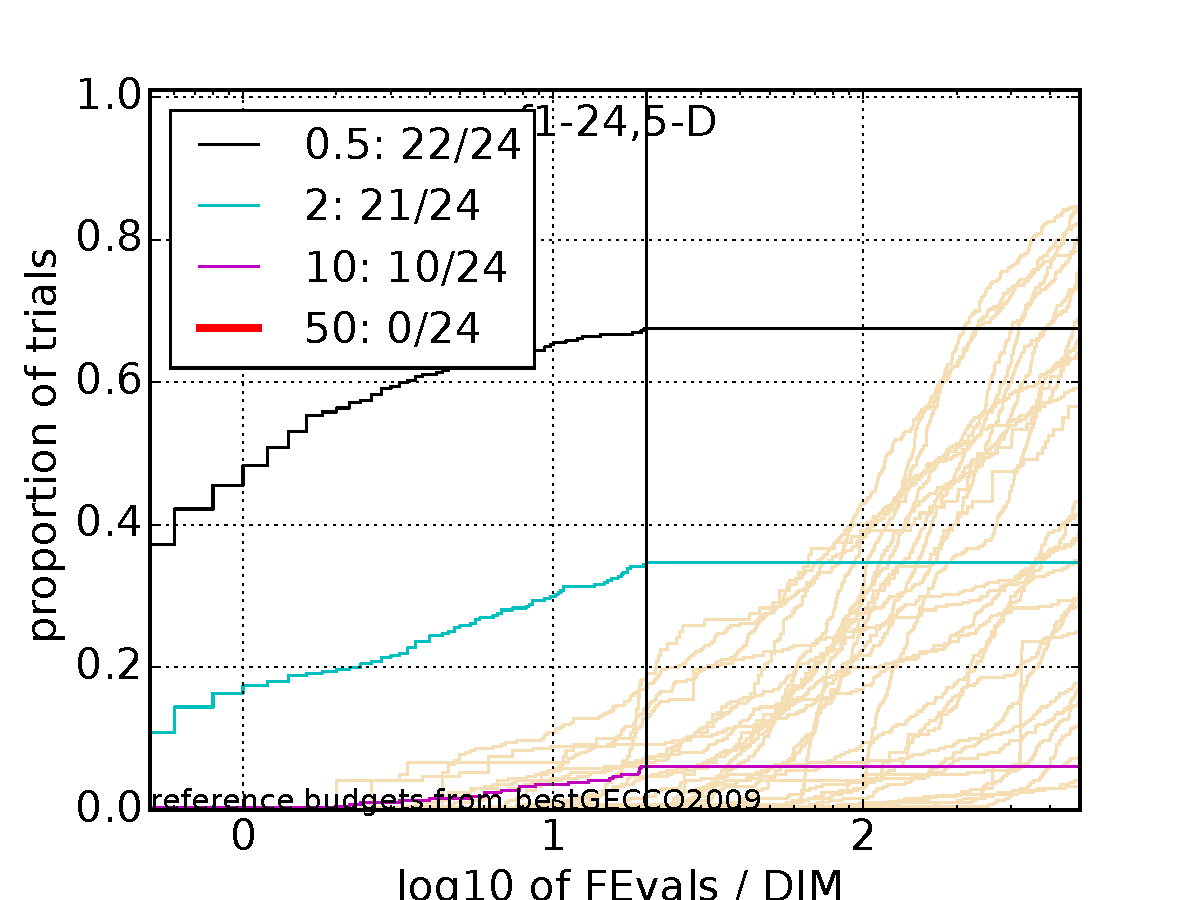
\includegraphics[width=0.528\textwidth,trim=0 0mm 16mm 11mm, clip]{pprldistr_05D_noiselessall} &
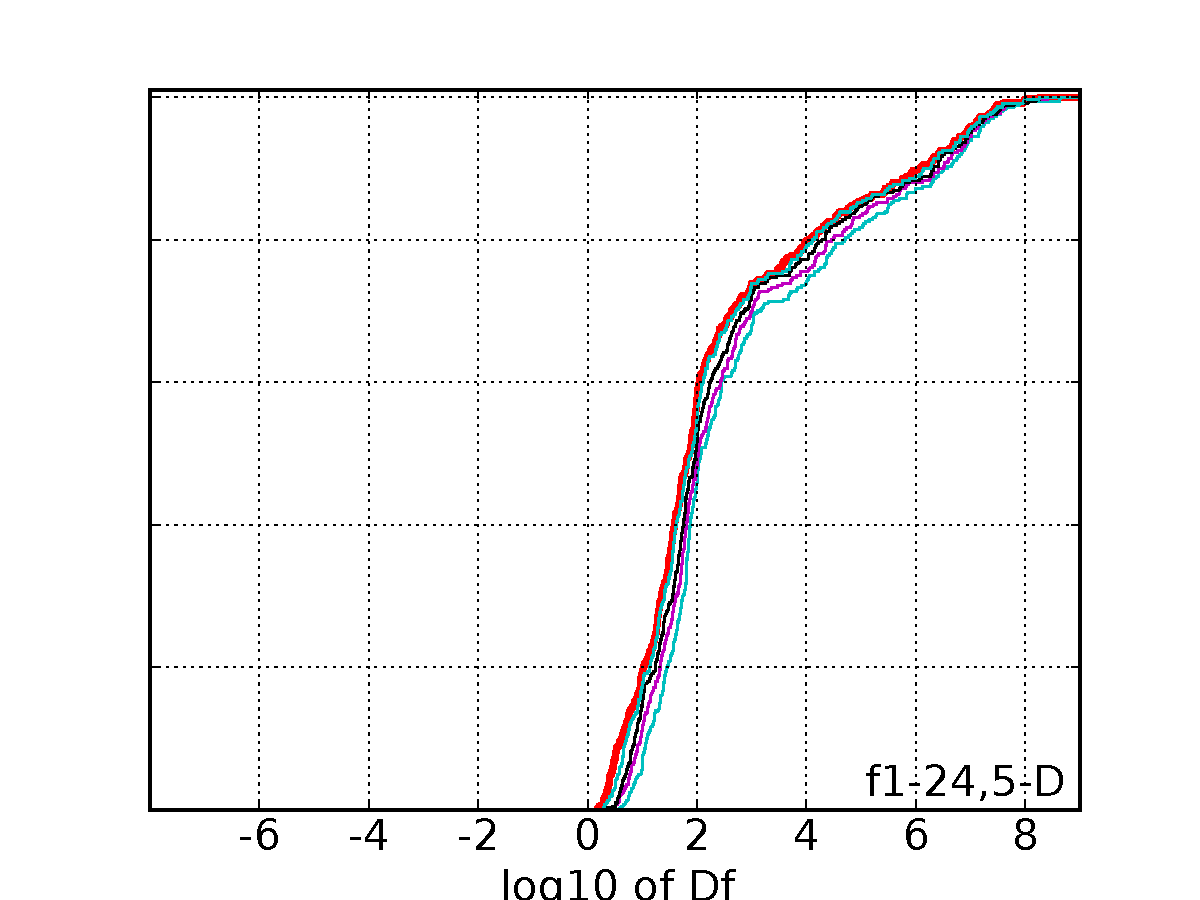
\includegraphics[width=0.46\textwidth,trim=24mm 0mm 16mm 11mm, clip]{ppfvdistr_05D_noiselessall}\\
\rot[5]{all functions}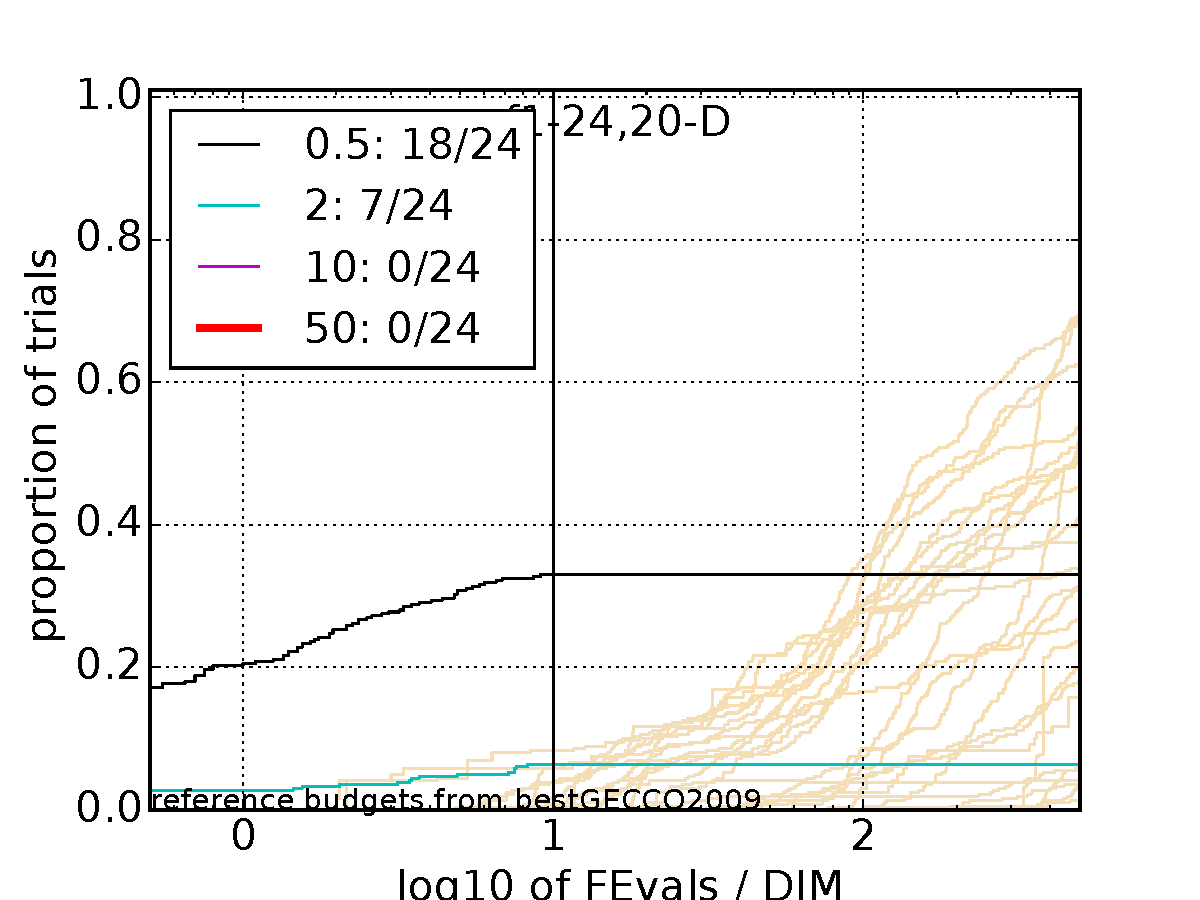
\includegraphics[width=0.528\textwidth,trim=0 0mm 16mm 11mm, clip]{pprldistr_20D_noiselessall} &
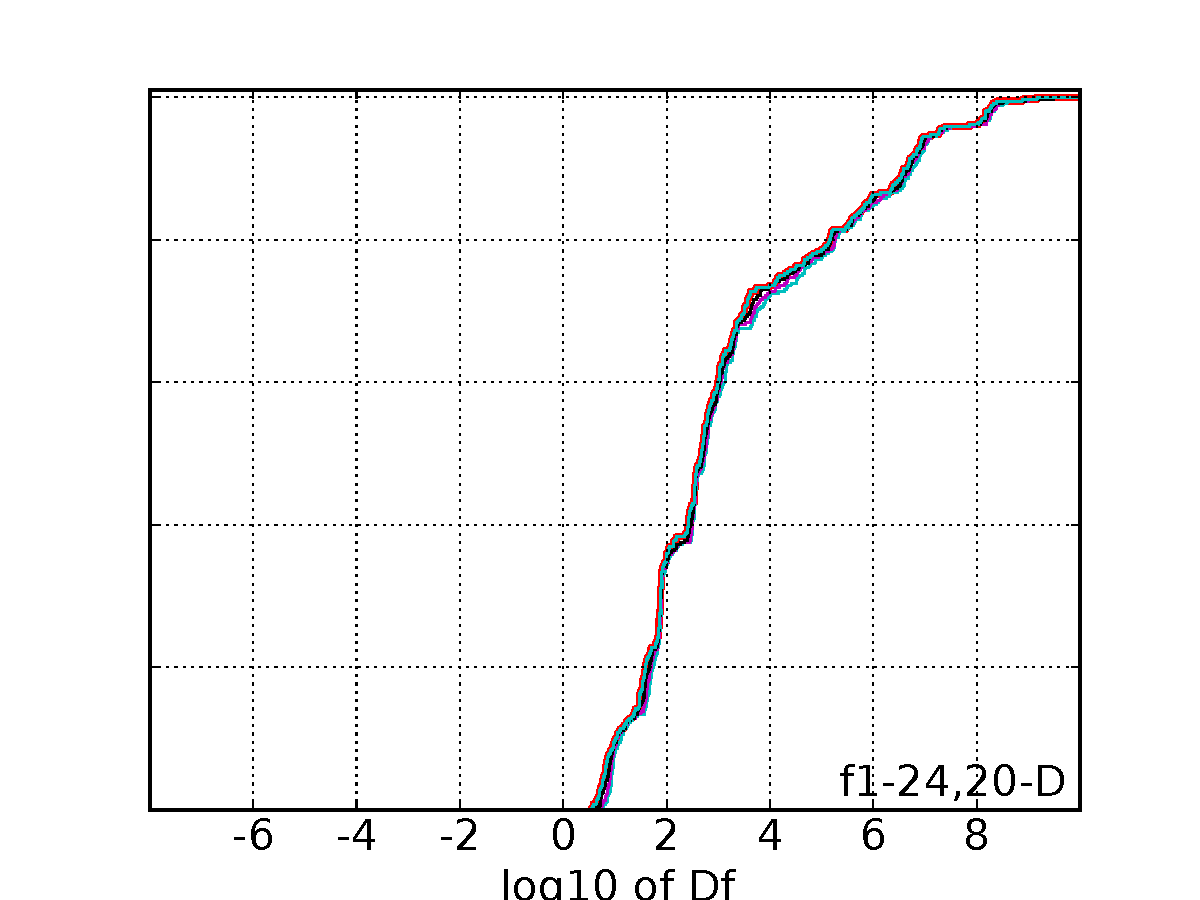
\includegraphics[width=0.46\textwidth,trim=24mm 0mm 16mm 11mm, clip]{ppfvdistr_20D_noiselessall}
\end{tabular}
\caption{\label{fig:RLDs05Da\algfolder} \bbobpprldistrlegend{} The top row shows results for 5-D and the bottom row for 20-D.}
\end{figure}
%%%%%%%%%%%%%%%%%%%%%%%%%%%%%%%%%%%%%%%%%%%%%%%%%%%%%%%%%%%%%%%%%%%%%%%%%%%%%%%
%%%%%%%%%%%%%%%%%%%%%%%%%%%%%%%%%%%%%%%%%%%%%%%%%%%%%%%%%%%%%%%%%%%%%%%%%%%%%%%
\begin{figure}[htbp!]
\centering
\begin{tabular}{@{}c@{}c@{}}
\rot[2.5]{separable fcts}
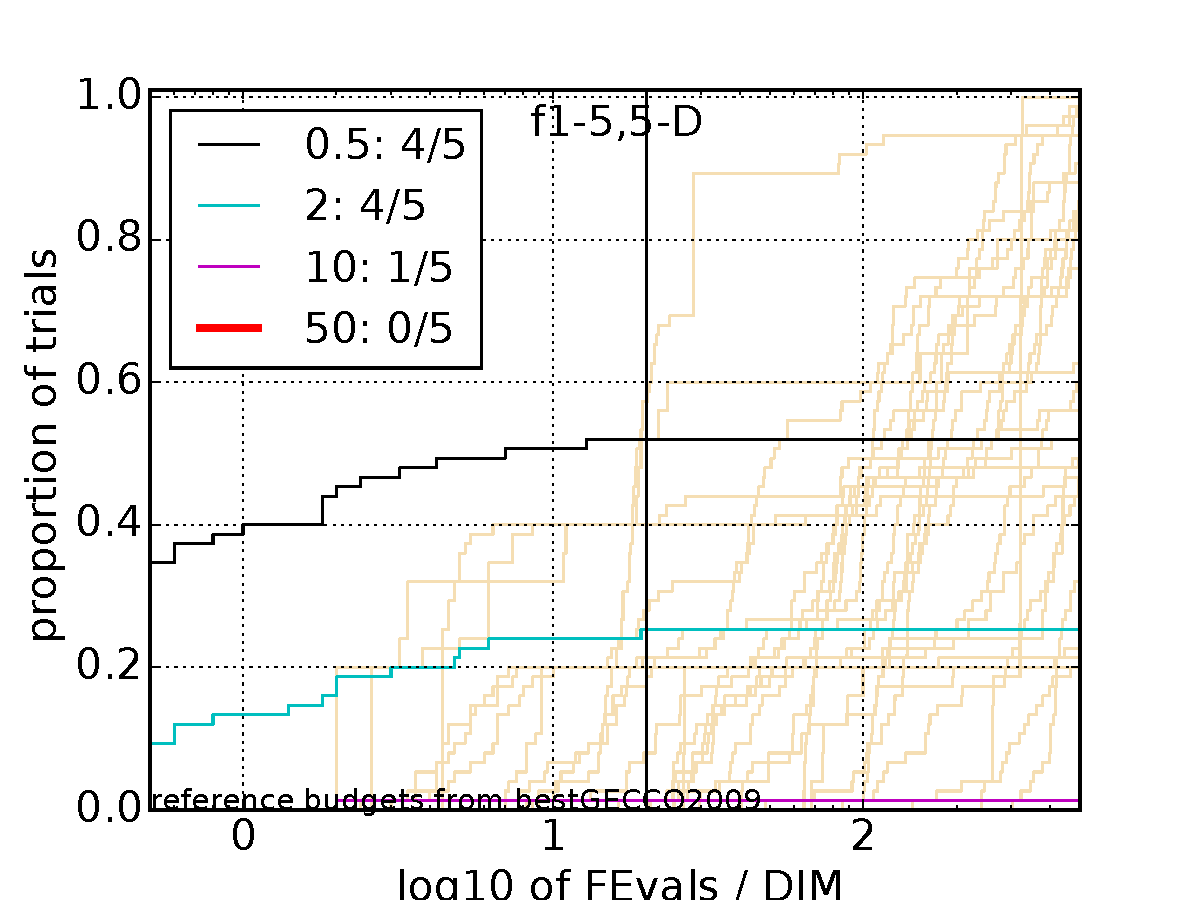
\includegraphics[width=0.41\textwidth,trim=0 7.5mm 16mm 11mm, clip]{pprldistr_05D_separ} &
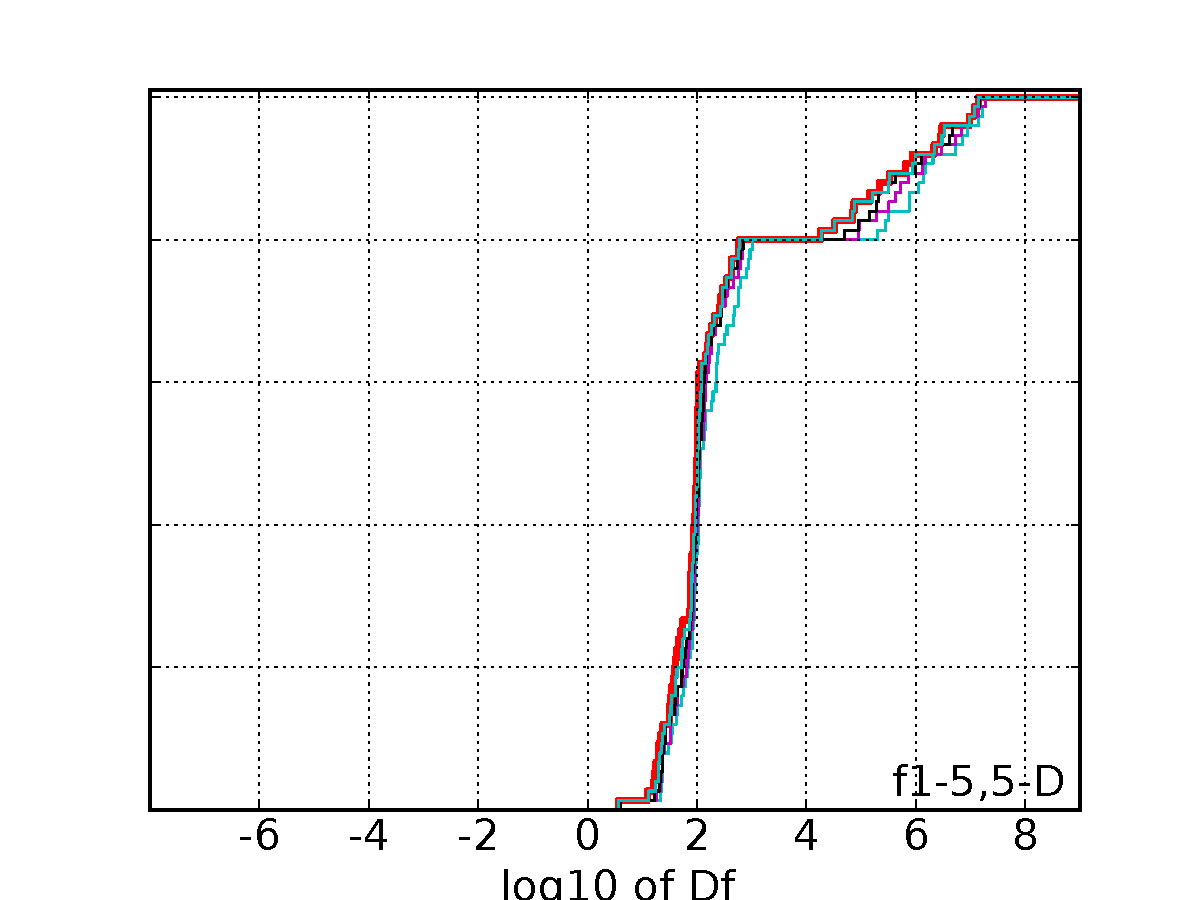
\includegraphics[width=0.3579\textwidth,trim=24mm 7.5mm 16mm 11mm, clip]{ppfvdistr_05D_separ}
\\[-1ex]
\rot[1.3]{misc.\ moderate fcts}
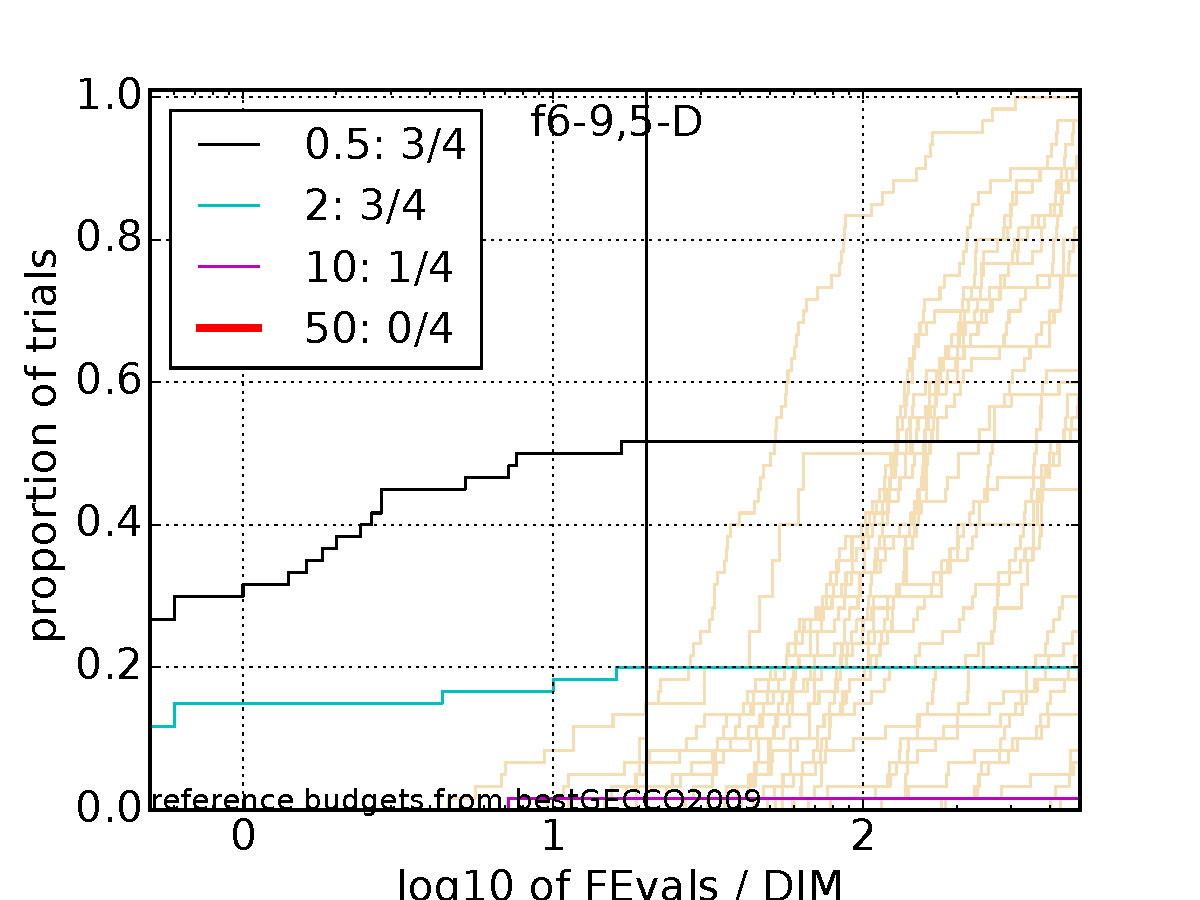
\includegraphics[width=0.41\textwidth,trim=0 7.5mm 16mm 11mm, clip]{pprldistr_05D_lcond} &
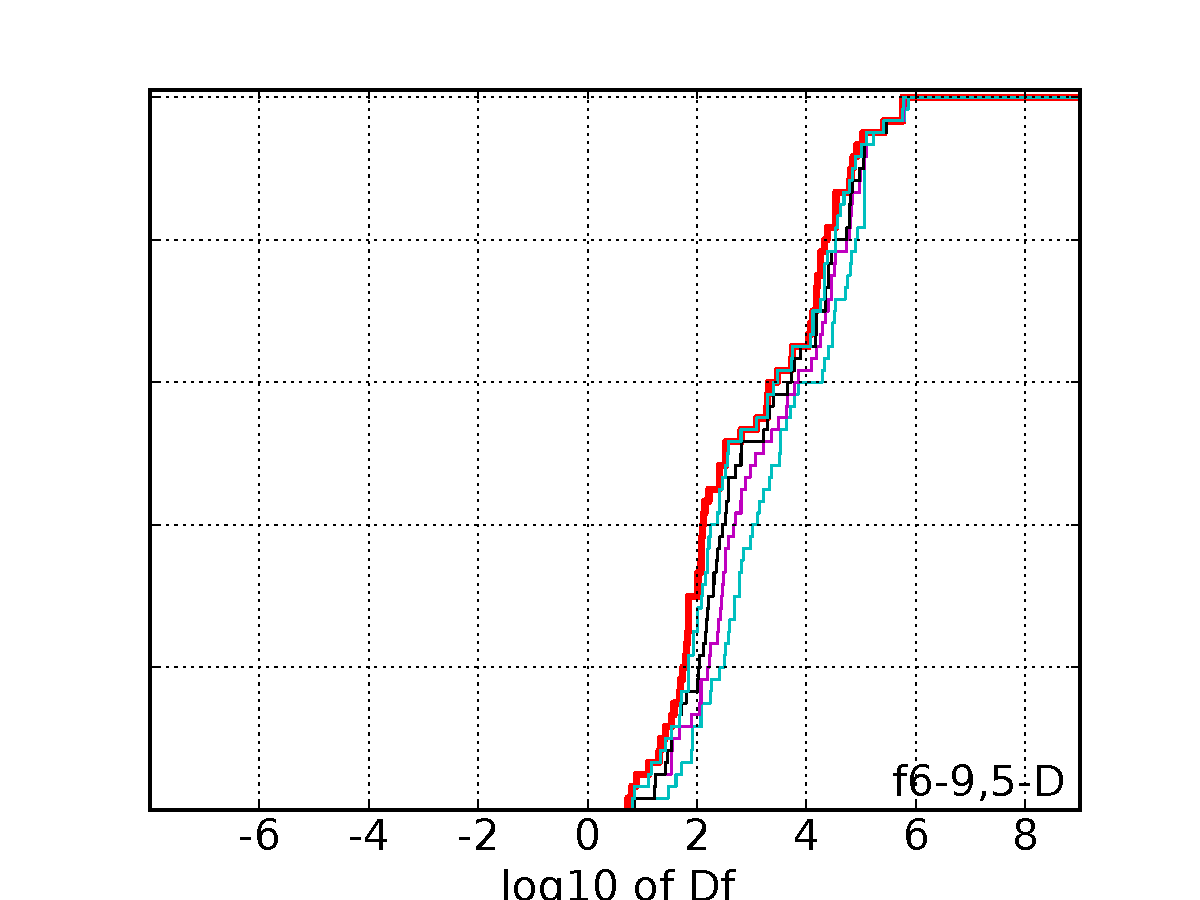
\includegraphics[width=0.3579\textwidth,trim=24mm 7.5mm 16mm 11mm, clip]{ppfvdistr_05D_lcond}
\\[-1ex]
\rot[1.1]{ill-conditioned fcts}
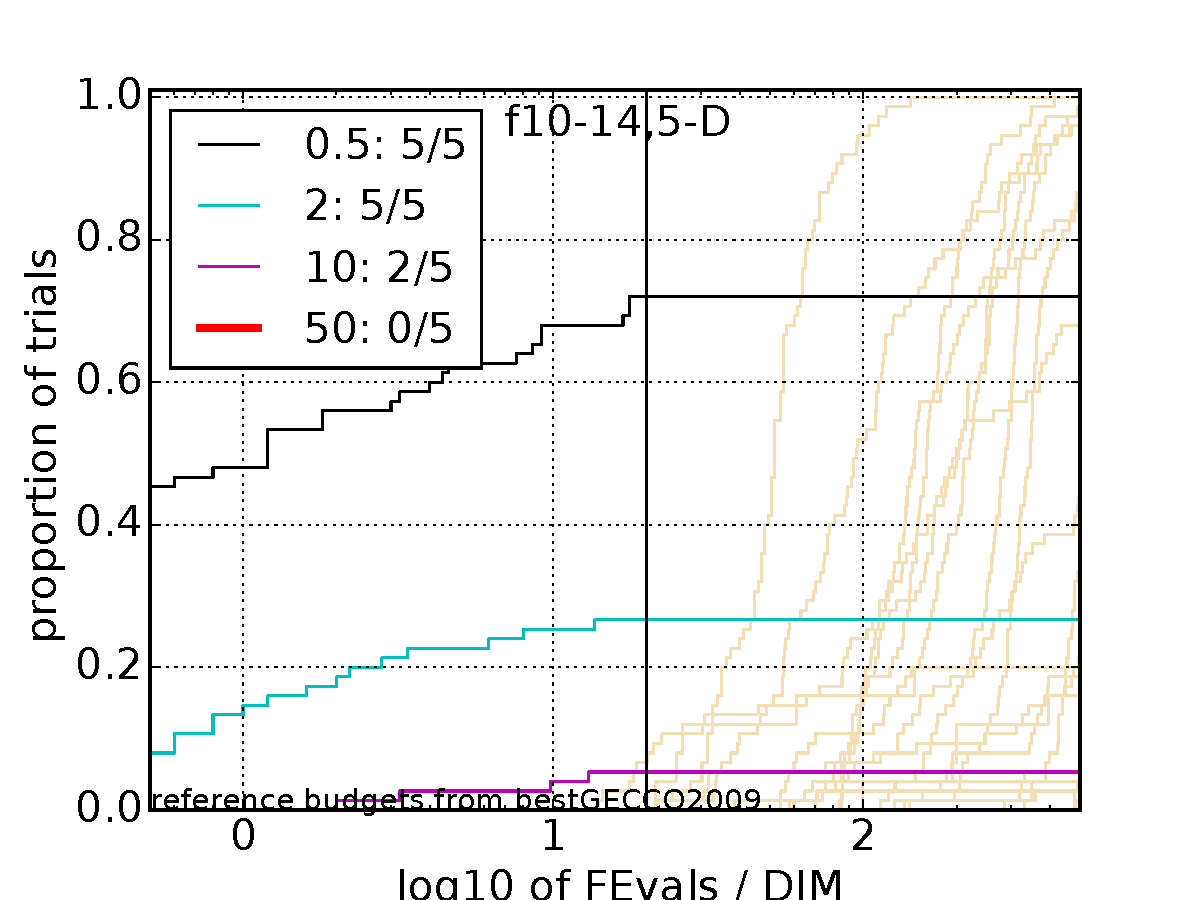
\includegraphics[width=0.41\textwidth,trim=0 7.5mm 16mm 11mm, clip]{pprldistr_05D_hcond} &
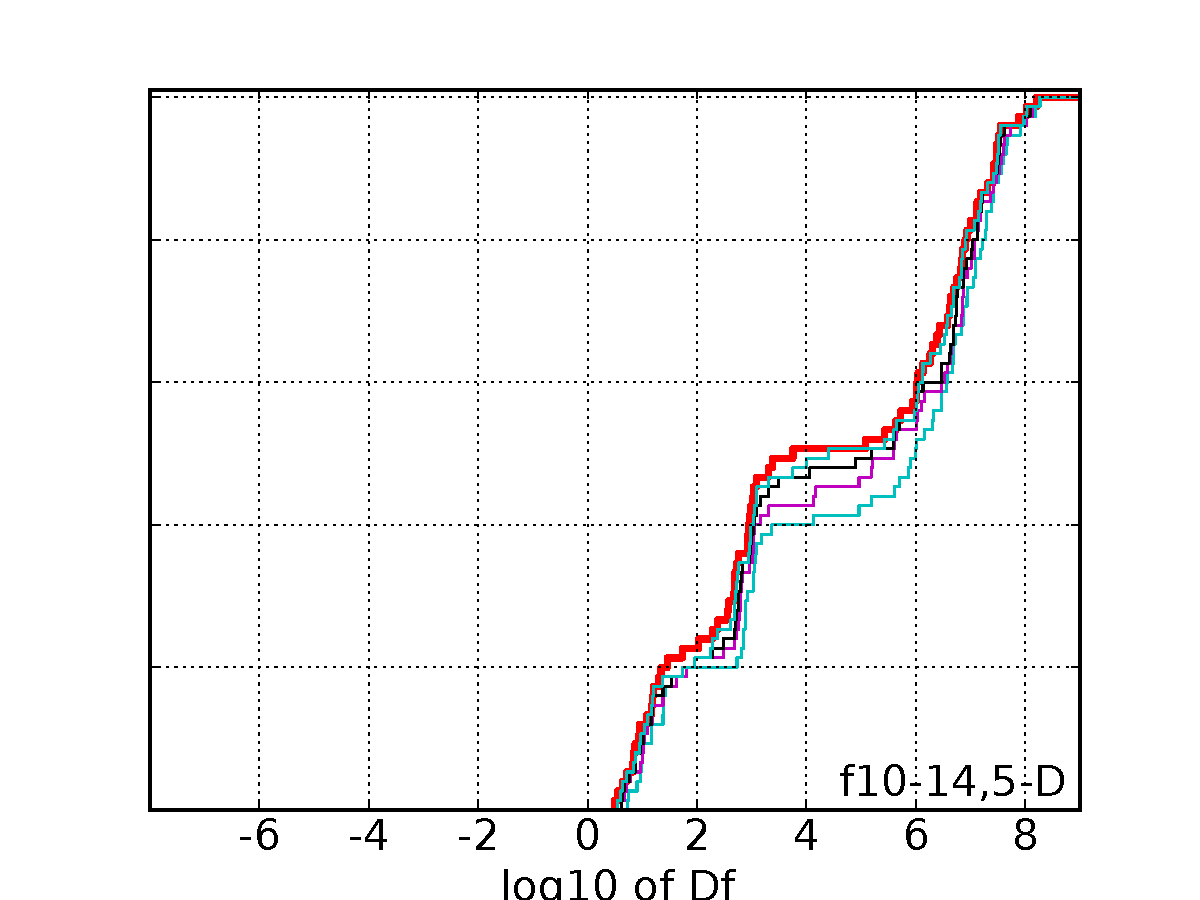
\includegraphics[width=0.3579\textwidth,trim=24mm 7.5mm 16mm 11mm, clip]{ppfvdistr_05D_hcond}
\\[-1ex]
\rot[1.7]{multi-modal fcts}
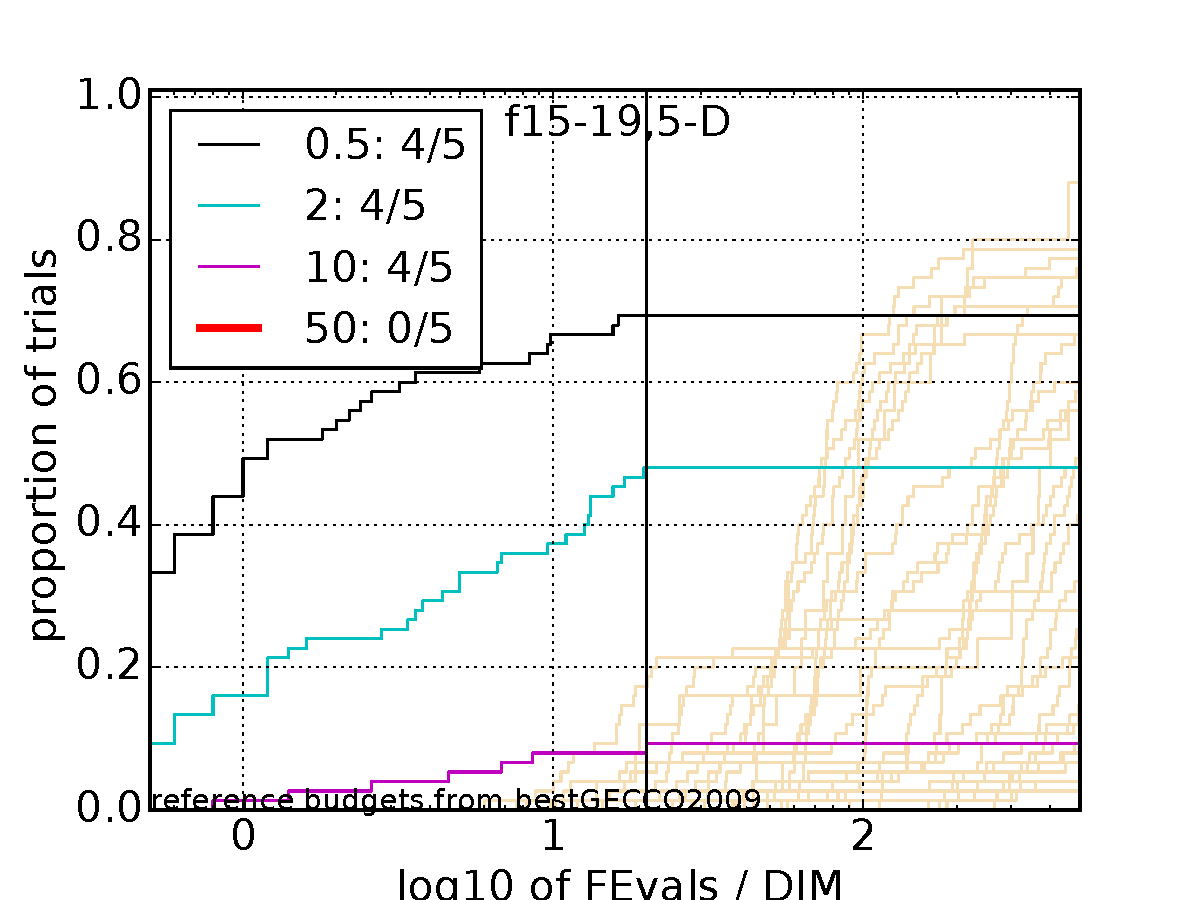
\includegraphics[width=0.41\textwidth,trim=0 7.5mm 16mm 11mm, clip]{pprldistr_05D_multi} &
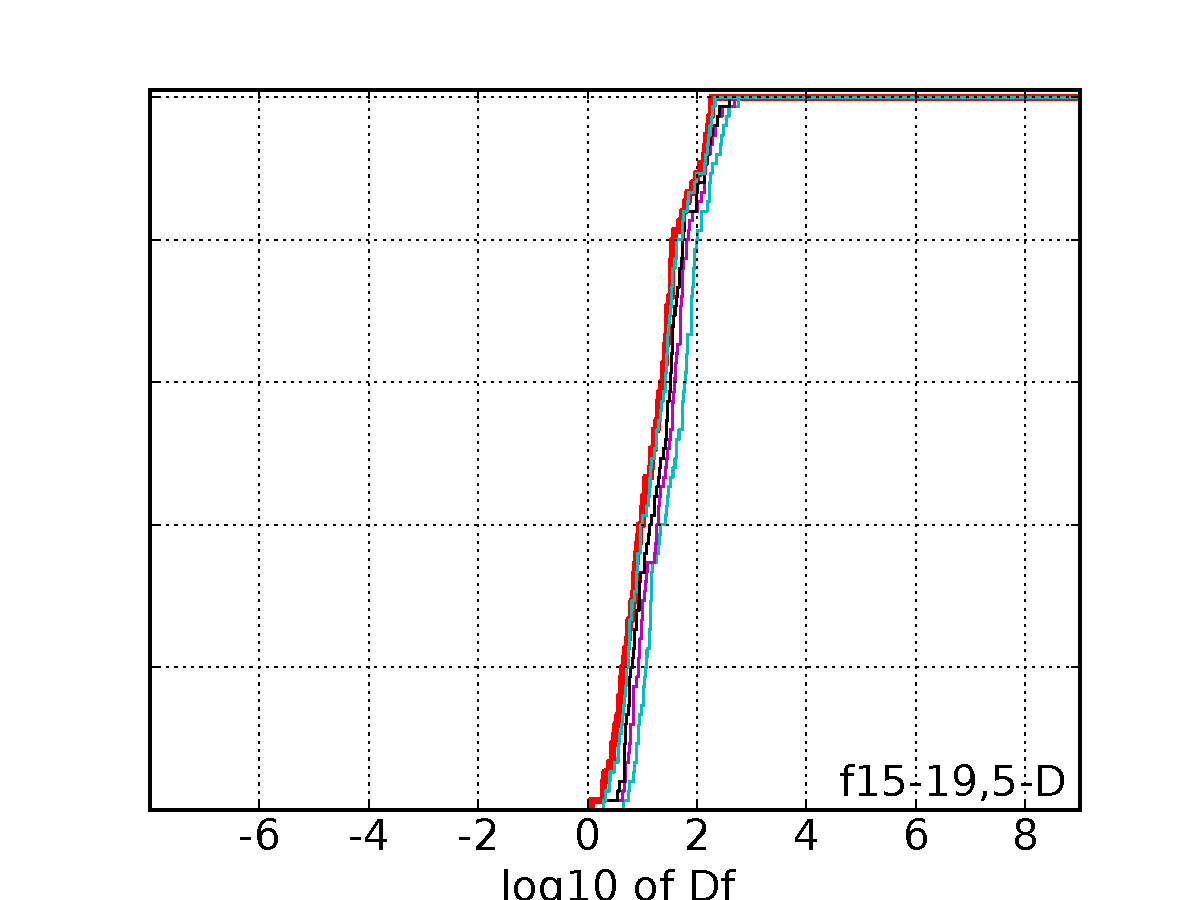
\includegraphics[width=0.3579\textwidth,trim=24mm 7.5mm 16mm 11mm, clip]{ppfvdistr_05D_multi}
\\[-1ex]
\rot[1.5]{weak structure fcts}
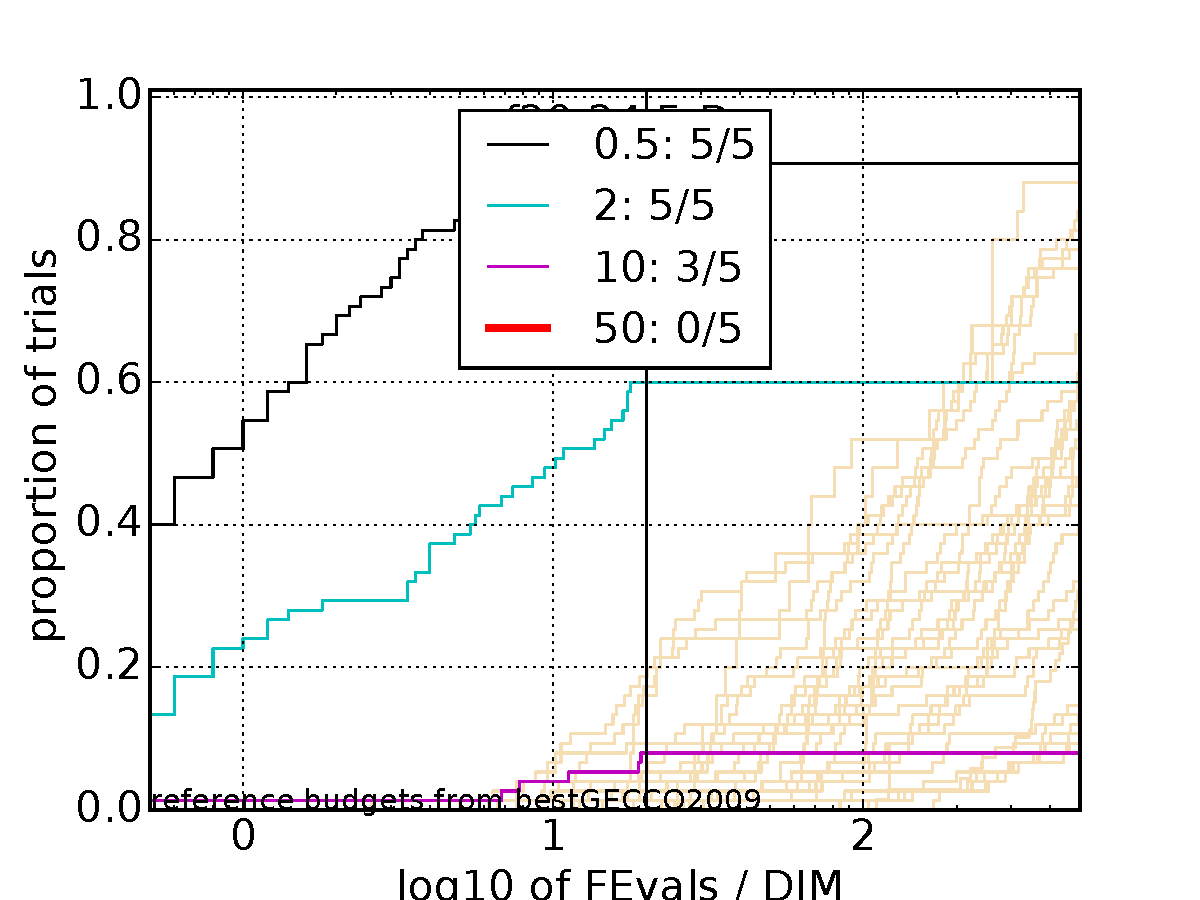
\includegraphics[width=0.41\textwidth,trim=0 0mm 16mm 11mm, clip]{pprldistr_05D_mult2} &
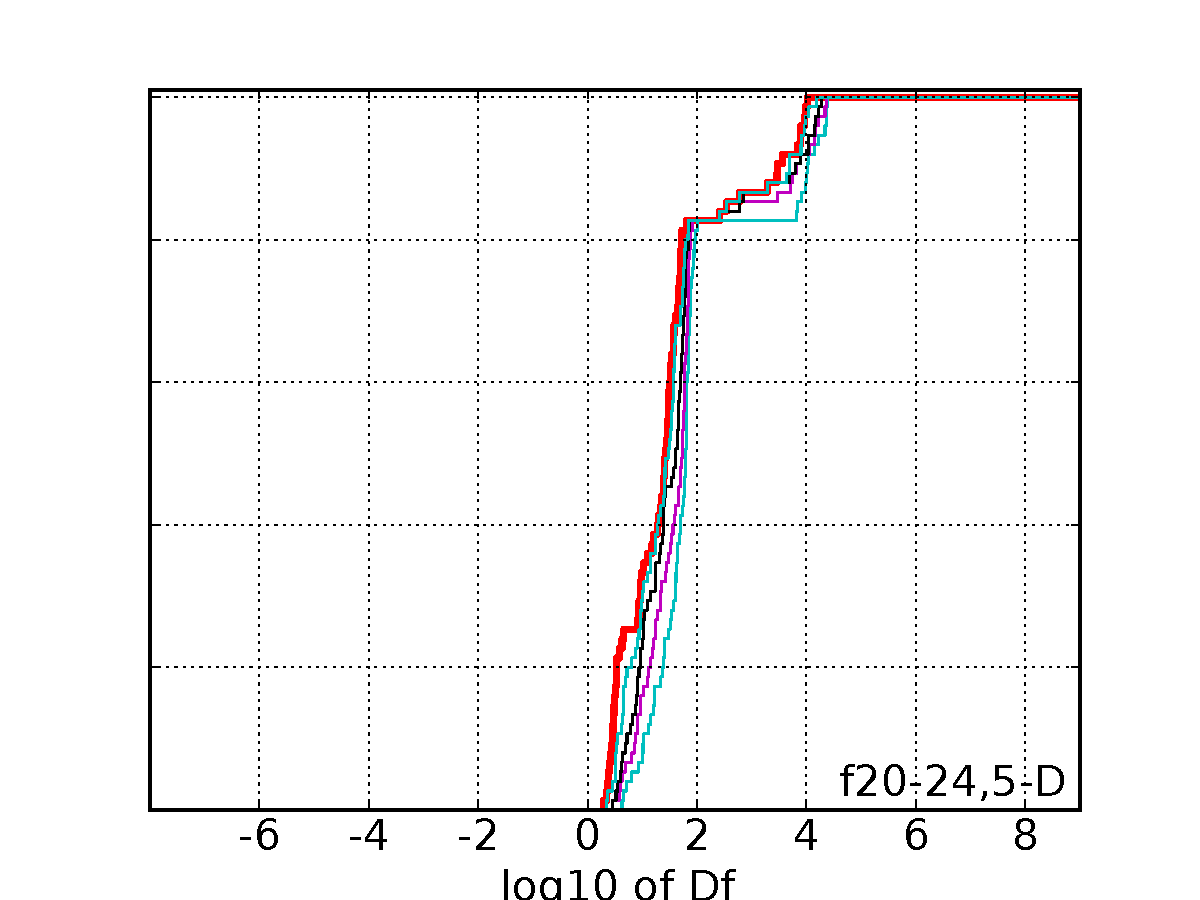
\includegraphics[width=0.3579\textwidth,trim=24mm 0mm 16mm 11mm, clip]{ppfvdistr_05D_mult2}
\end{tabular}
\vspace*{-0.5ex}
\caption{\label{fig:RLDs05Db\algfolder}Subgroups of functions 5-D. See caption of Figure~\ref{fig:RLDs05Da\algfolder} for details.
%Left subplots: Empirical Cumulative Distribution Function (ECDF) of the running time (number of function evaluations),
%divided by search space dimension $D$, to fall below $\fopt+\Df$ with
%$\Df=10^{k}$, where $k$ is the first value in the legend. The vertical black
%line indicates the maximum number of function evaluations. The legends indicate
%the number of functions that were solved in at least one trial.
%% FEvals denotes number of function evaluations,
%Light brown lines in the background show ECDFs for target value $10^{-8}$ of
%all algorithms benchmarked during BBOB 2009. Right subplots: ECDF of
%the best achieved \Df\ divided by $10^k$ (upper left lines in continuation of
%the left subplot), and best achieved \Df\ divided by $10^{-8}$ for running
%times of $D, 10\,D, 100\,D\dots$ function evaluations (from right to left
%cycling black-cyan-magenta).
%%Top row: all functions; second row: separable
%%functions; third row: misc.\ moderate functions; fourth row:
%%ill-conditioned functions; fifth row: multi-modal functions with
%%adequate structure; last row: multi-modal functions with weak structure.
%$D=\mathsf{DIM}$ denotes search space dimension (5 in this case) and $\Df=\mathsf{Df}$
%denotes the difference to the optimal function value.
}
\end{figure}
%%%%%%%%%%%%%%%%%%%%%%%%%%%%%%%%%%%%%%%%%%%%%%%%%%%%%%%%%%%%%%%%%%%%%%%%%%%%%%%
%%%%%%%%%%%%%%%%%%%%%%%%%%%%%%%%%%%%%%%%%%%%%%%%%%%%%%%%%%%%%%%%%%%%%%%%%%%%%%%
\begin{figure}[htbp!]
\centering
\begin{tabular}{@{}c@{}c@{}}
\rot[2.5]{separable fcts}
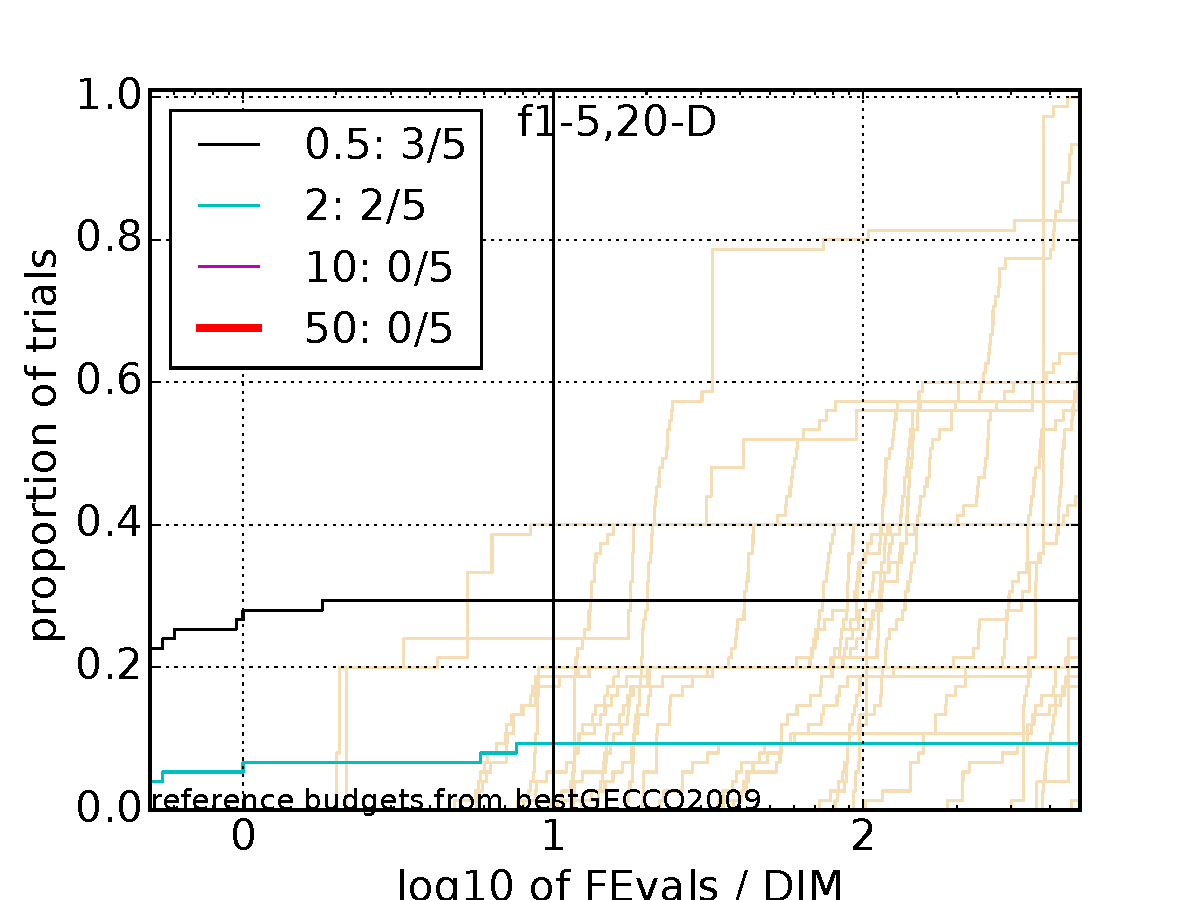
\includegraphics[width=0.41\textwidth,trim=0 7.5mm 16mm 11mm, clip]{pprldistr_20D_separ} &
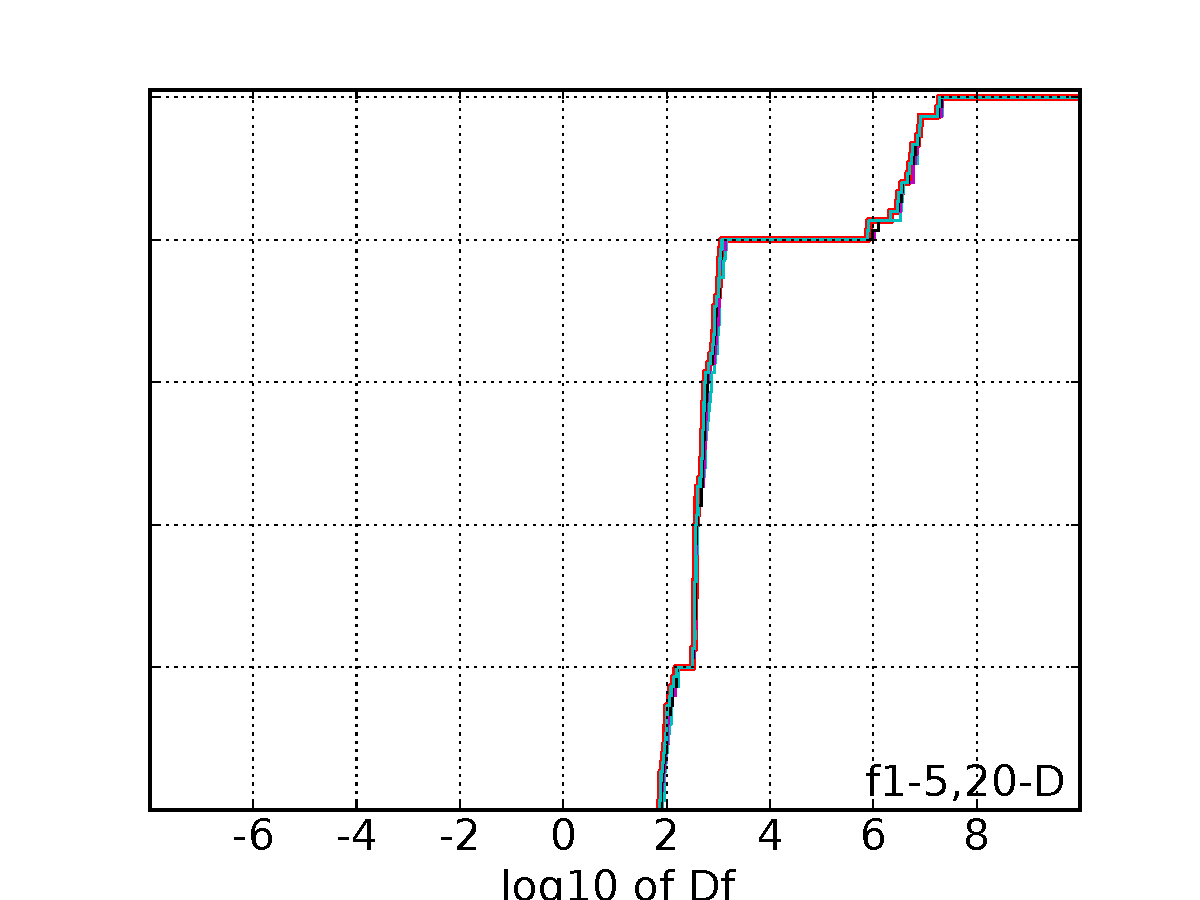
\includegraphics[width=0.3579\textwidth,trim=24mm 7.5mm 16mm 11mm, clip]{ppfvdistr_20D_separ}
\\[-1ex]
\rot[1.3]{misc.\ moderate fcts}
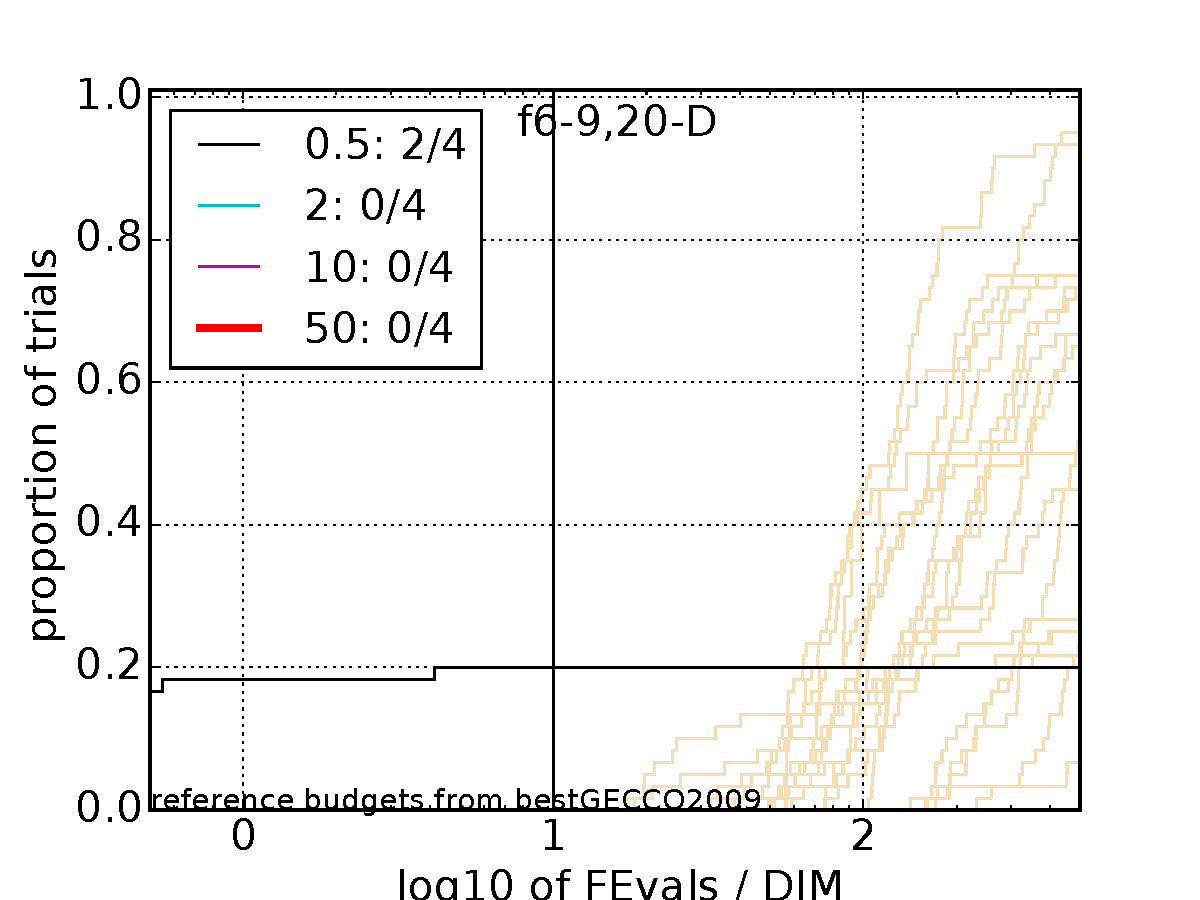
\includegraphics[width=0.41\textwidth,trim=0 7.5mm 16mm 11mm, clip]{pprldistr_20D_lcond} &
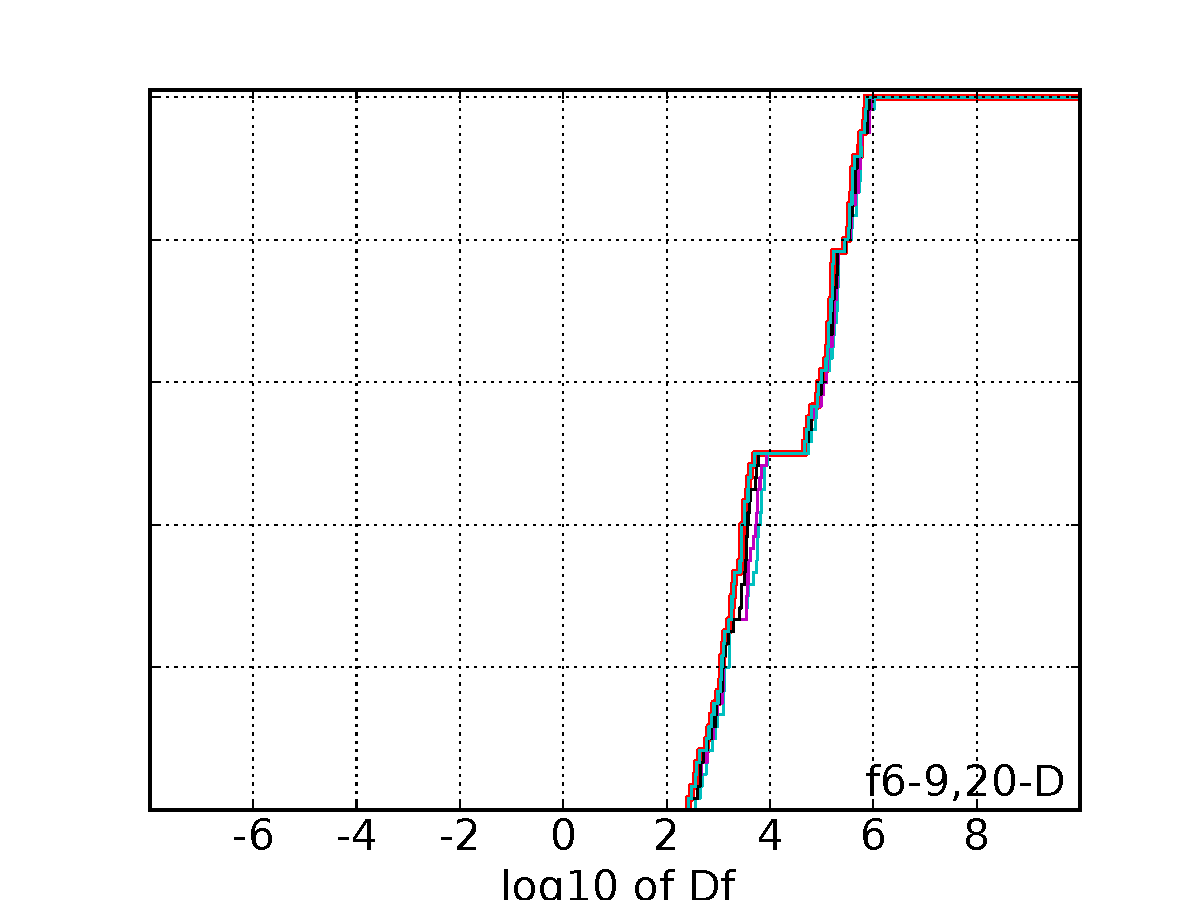
\includegraphics[width=0.3579\textwidth,trim=24mm 7.5mm 16mm 11mm, clip]{ppfvdistr_20D_lcond}
\\[-1ex]
\rot[1.1]{ill-conditioned fcts}
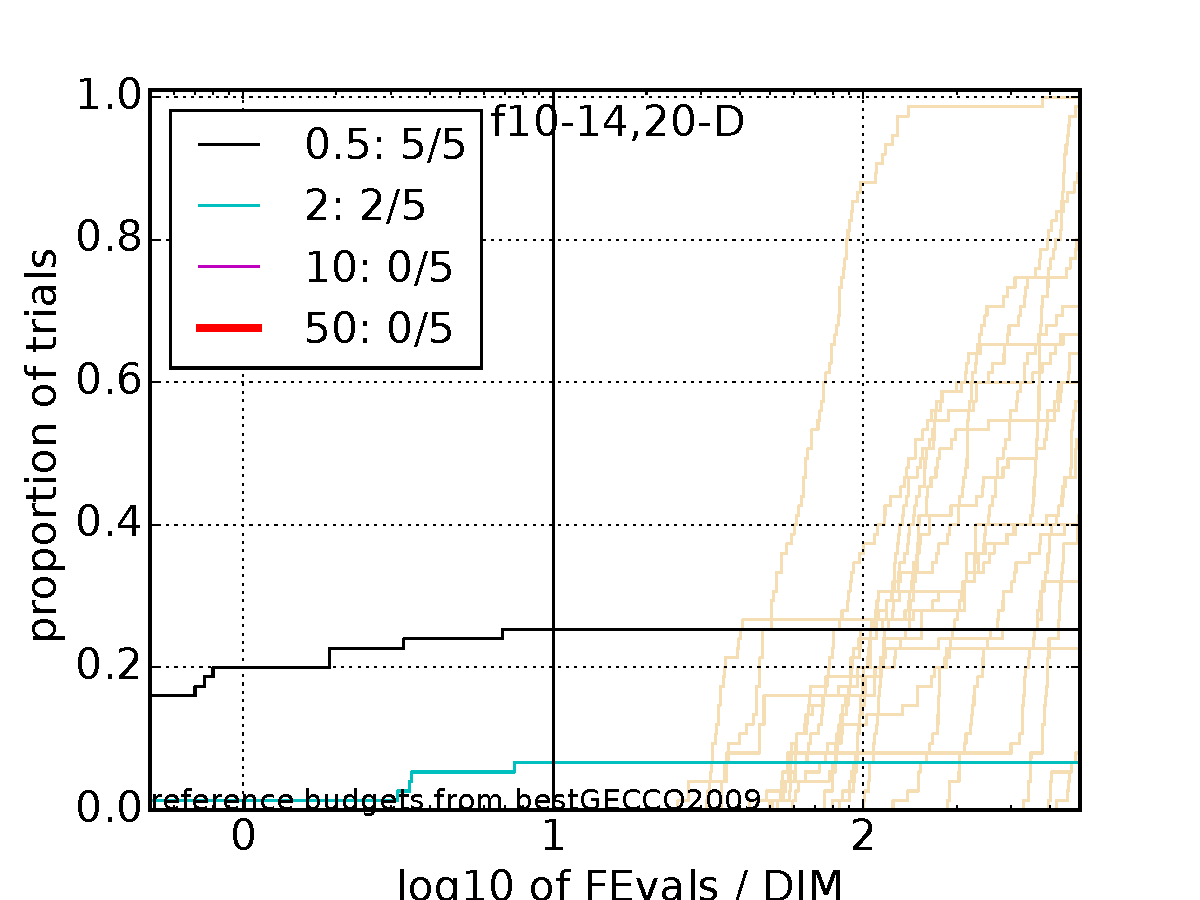
\includegraphics[width=0.41\textwidth,trim=0 7.5mm 16mm 11mm, clip]{pprldistr_20D_hcond} &
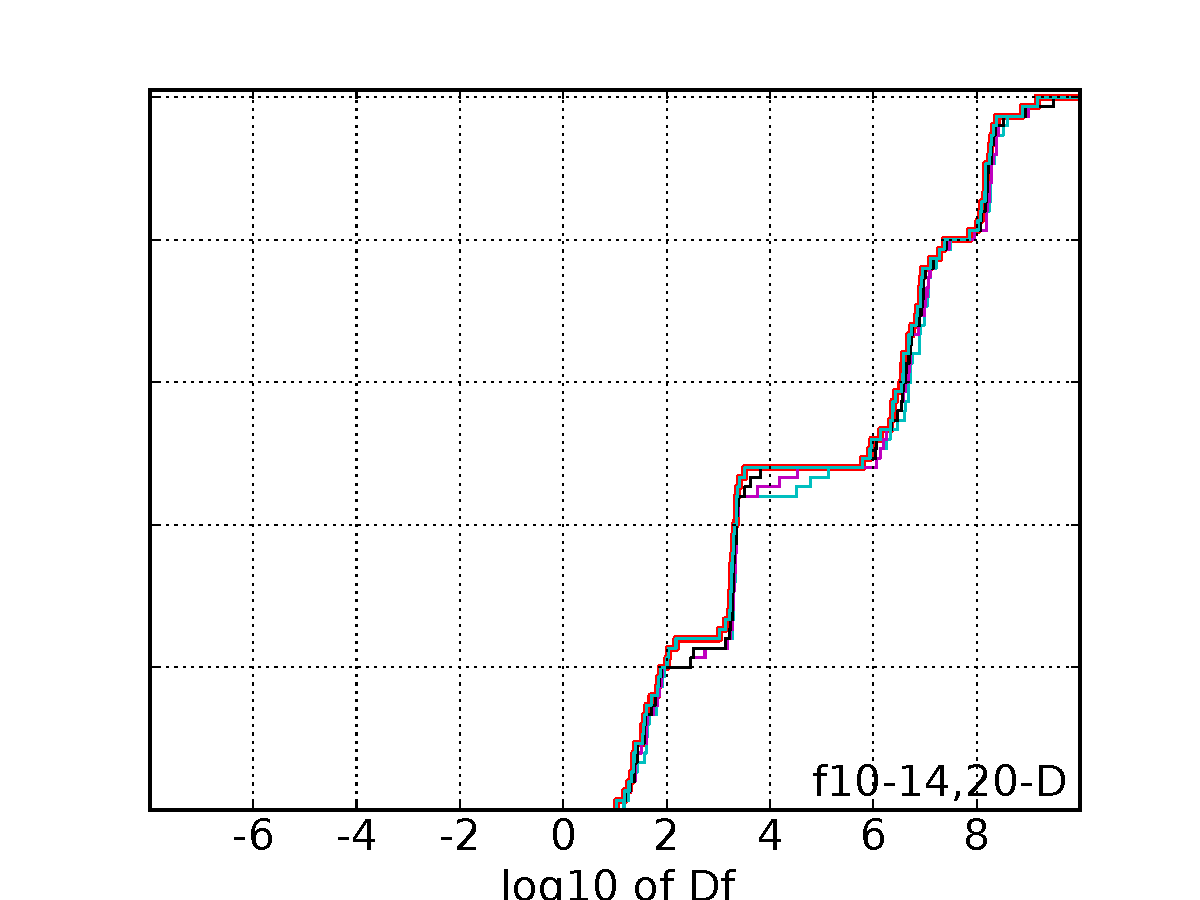
\includegraphics[width=0.3579\textwidth,trim=24mm 7.5mm 16mm 11mm, clip]{ppfvdistr_20D_hcond}
\\[-1ex]
\rot[1.7]{multi-modal fcts}
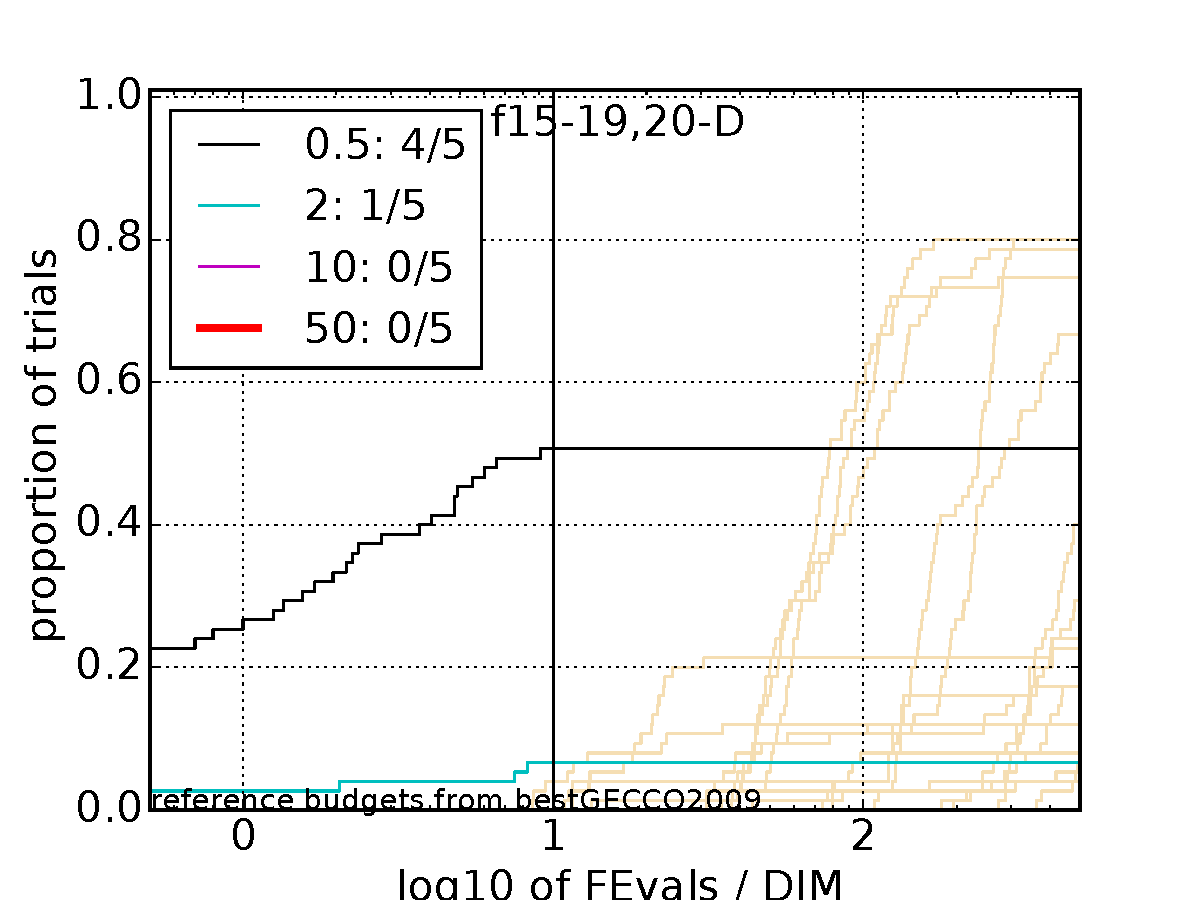
\includegraphics[width=0.41\textwidth,trim=0 7.5mm 16mm 11mm, clip]{pprldistr_20D_multi} &
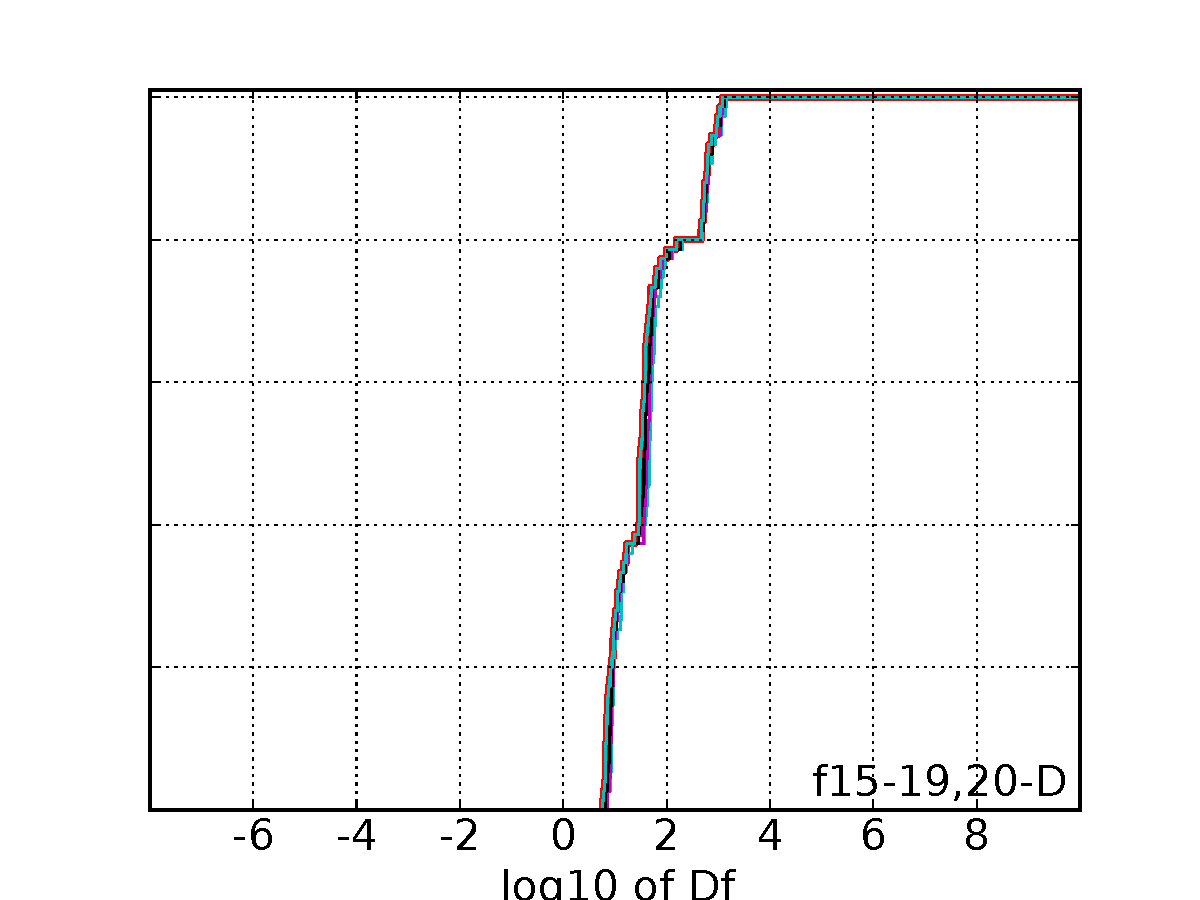
\includegraphics[width=0.3579\textwidth,trim=24mm 7.5mm 16mm 11mm, clip]{ppfvdistr_20D_multi}
\\[-1ex]
\rot[1.5]{weak structure fcts}
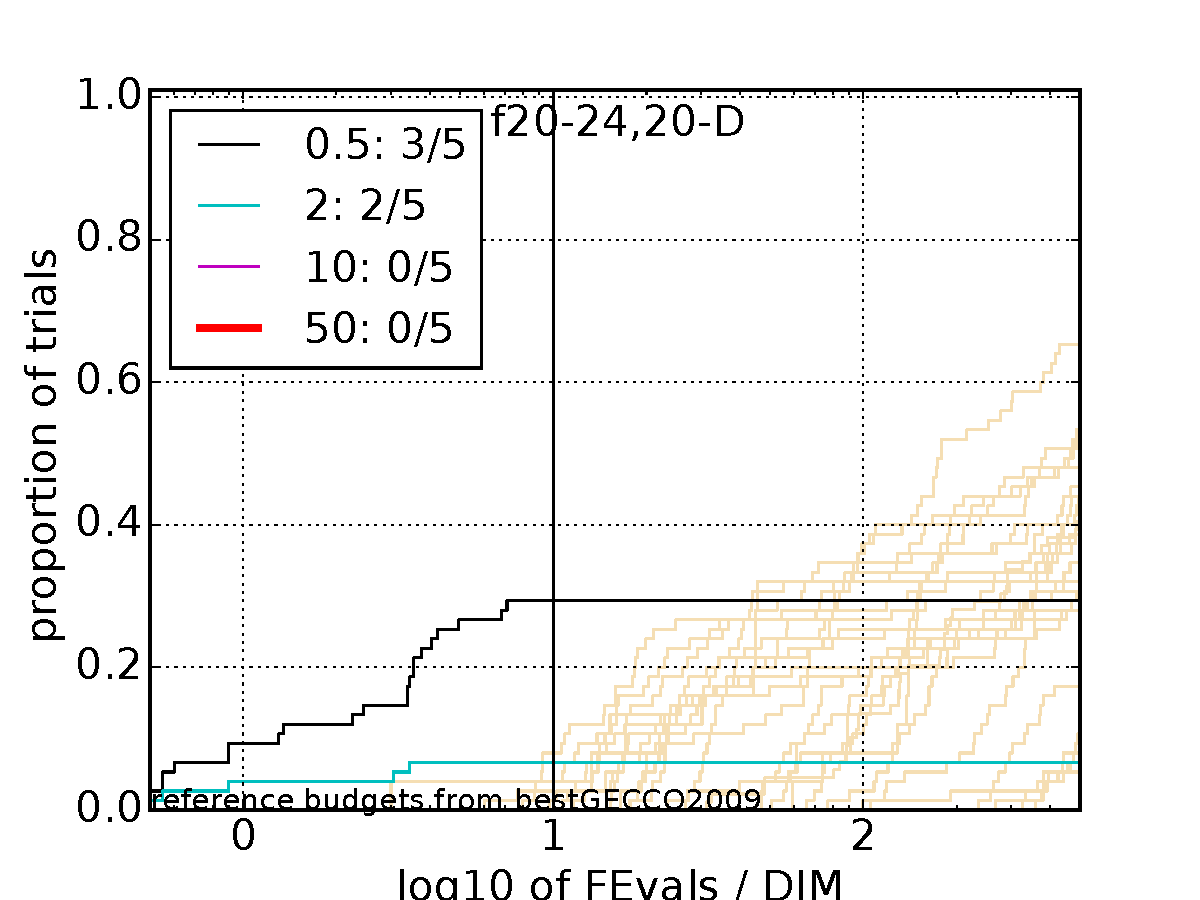
\includegraphics[width=0.41\textwidth,trim=0 0mm 16mm 11mm, clip]{pprldistr_20D_mult2} &
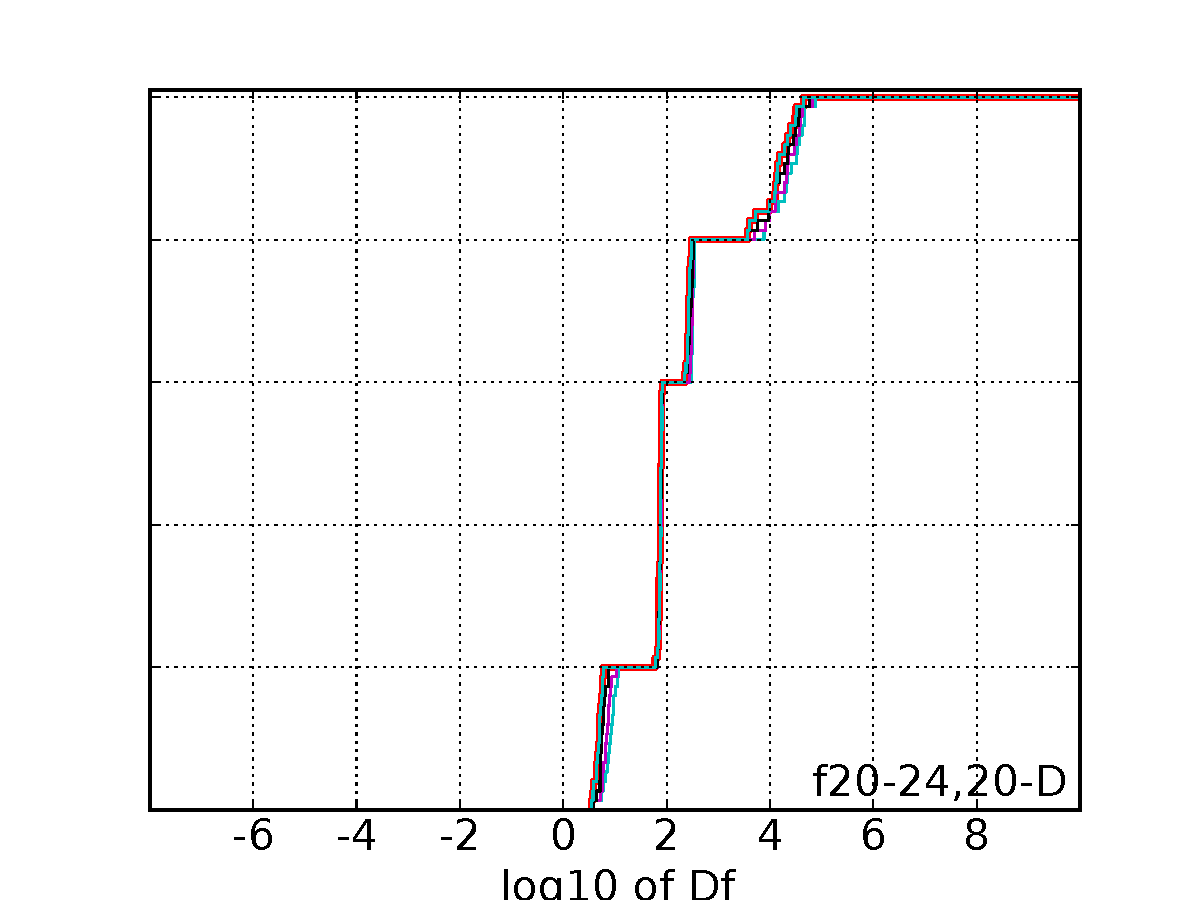
\includegraphics[width=0.3579\textwidth,trim=24mm 0mm 16mm 11mm, clip]{ppfvdistr_20D_mult2}
\end{tabular}
\vspace*{-0.5ex}
\caption{\label{fig:RLDs20Db\algfolder}Subgroups of functions 20-D. See caption
of Figure~\ref{fig:RLDs05Da\algfolder} for details.}
\end{figure}
%%%%%%%%%%%%%%%%%%%%%%%%%%%%%%%%%%%%%%%%%%%%%%%%%%%%%%%%%%%%%%%%%%%%%%%%%%%%%%%
%%%%%%%%%%%%%%%%%%%%%%%%%%%%%%%%%%%%%%%%%%%%%%%%%%%%%%%%%%%%%%%%%%%%%%%%%%%%%%%
\begin{figure}[htbp!]
\subfloat{
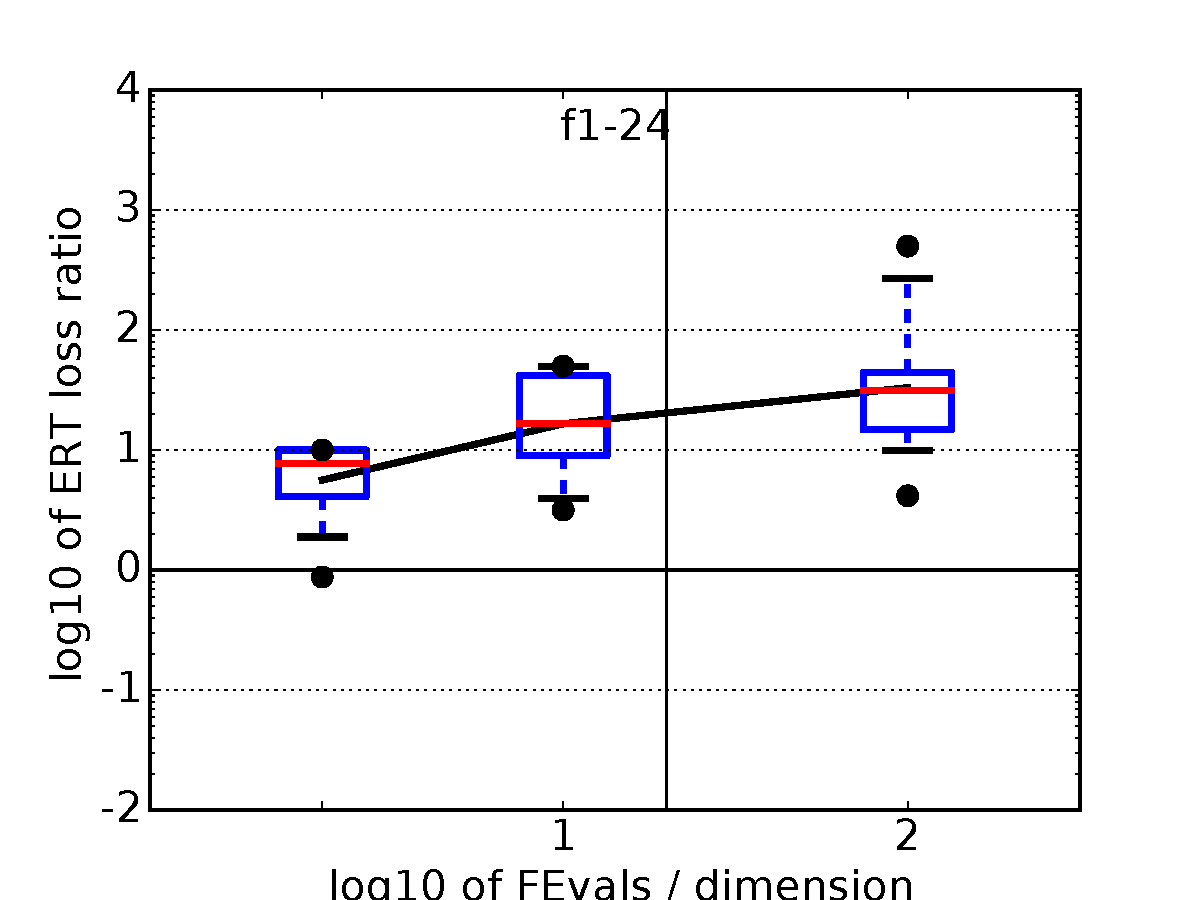
\includegraphics[width=0.35\textwidth,trim=9mm 8mm 18mm 12mm, clip]{pplogloss_05D_noiselessall}
}
\subfloat{
\centering
\scriptsize
\input{\bbobdatapath\algfolder pploglosstable_05D_noiselessall}}\\[-2ex]
\subfloat{
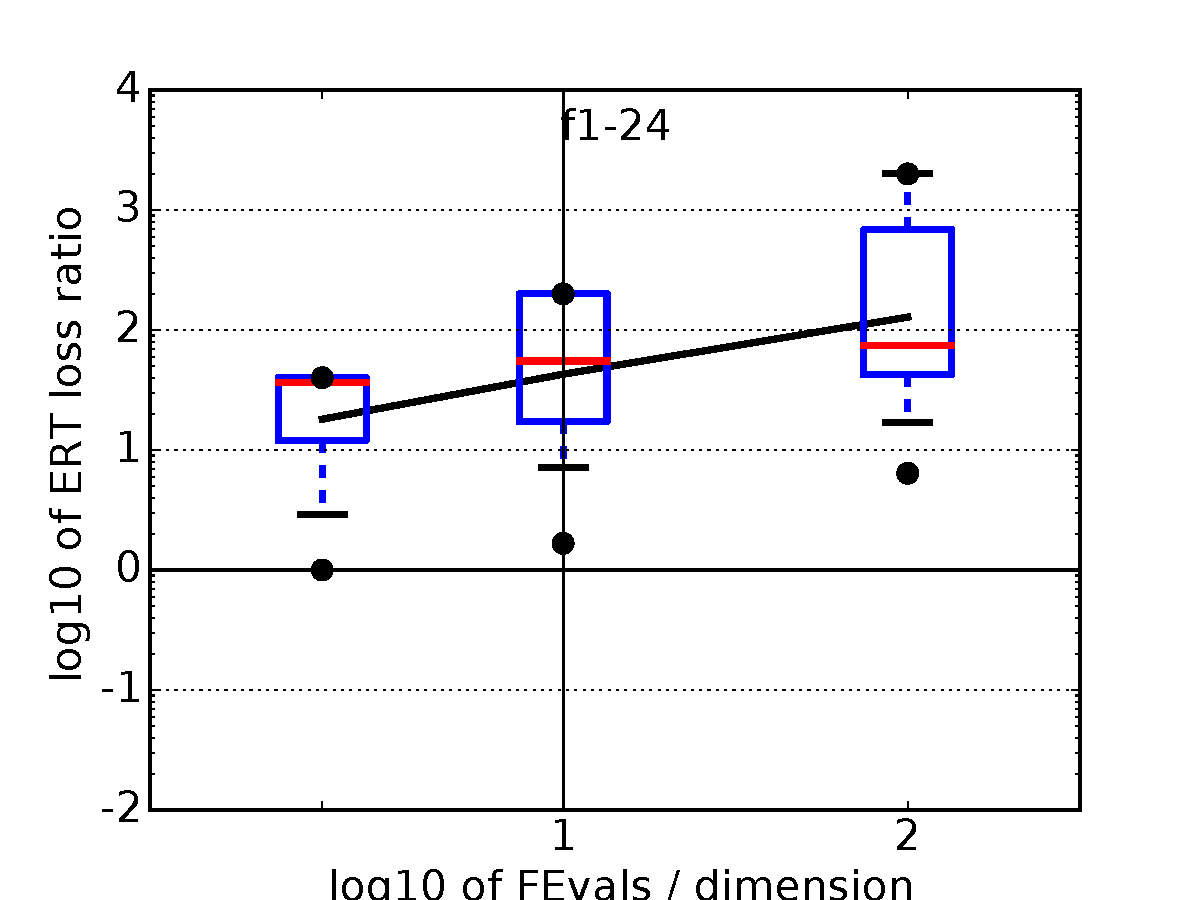
\includegraphics[width=0.35\textwidth,trim=9mm 0mm 18mm 12mm, clip]{pplogloss_20D_noiselessall}
}
\subfloat{
\centering
\scriptsize
\input{\bbobdatapath\algfolder pploglosstable_20D_noiselessall}}
\caption{\label{fig:ERTloglossa\algfolder}
\ERT\ loss ratio. Left: plotted versus given budget
$\FEvals=\nbFEs$ in log-log display. Box-Whisker plot shows 25-75\%-ile (box)
with median, 10-90\%-ile (caps), and minimum and maximum \ERT\ loss ratio
(points). The black line is the geometric mean. The vertical line gives the
maximal number of function evaluations. Right: tabulated \ERT\ loss ratios
in 5-D (top table) and 20-D (bottom table). maxFE/D gives the maximum number of
function evaluations divided by the dimension. RL$_{\text{US}}$/D gives the
median number of function evaluations for unsuccessful trials.}
\end{figure}
%%%%%%%%%%%%%%%%%%%%%%%%%%%%%%%%%%%%%%%%%%%%%%%%%%%%%%%%%%%%%%%%%%%%%%%%%%%%%%%
%%%%%%%%%%%%%%%%%%%%%%%%%%%%%%%%%%%%%%%%%%%%%%%%%%%%%%%%%%%%%%%%%%%%%%%%%%%%%%%
\begin{figure}[htbp!]
\centering
\begin{tabular}{@{}ll@{}}
\multicolumn{1}{c}{5-D} & \multicolumn{1}{c}{20-D}\\
%\rot{all functions}
%\hspace*{-2mm}
%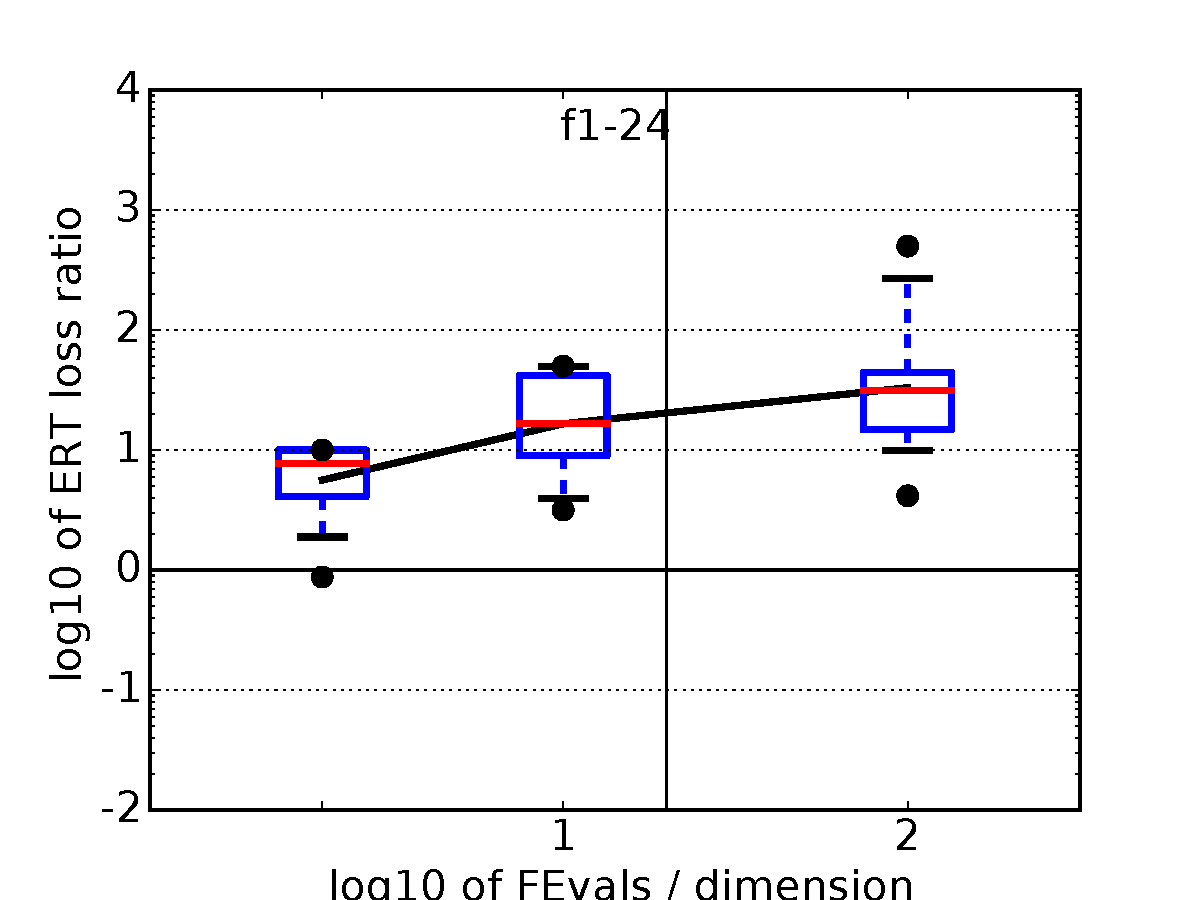
\includegraphics[width=0.24\textwidth,trim=0 0 16mm 12mm, clip]{pplogloss_05D_noiselessall} &
%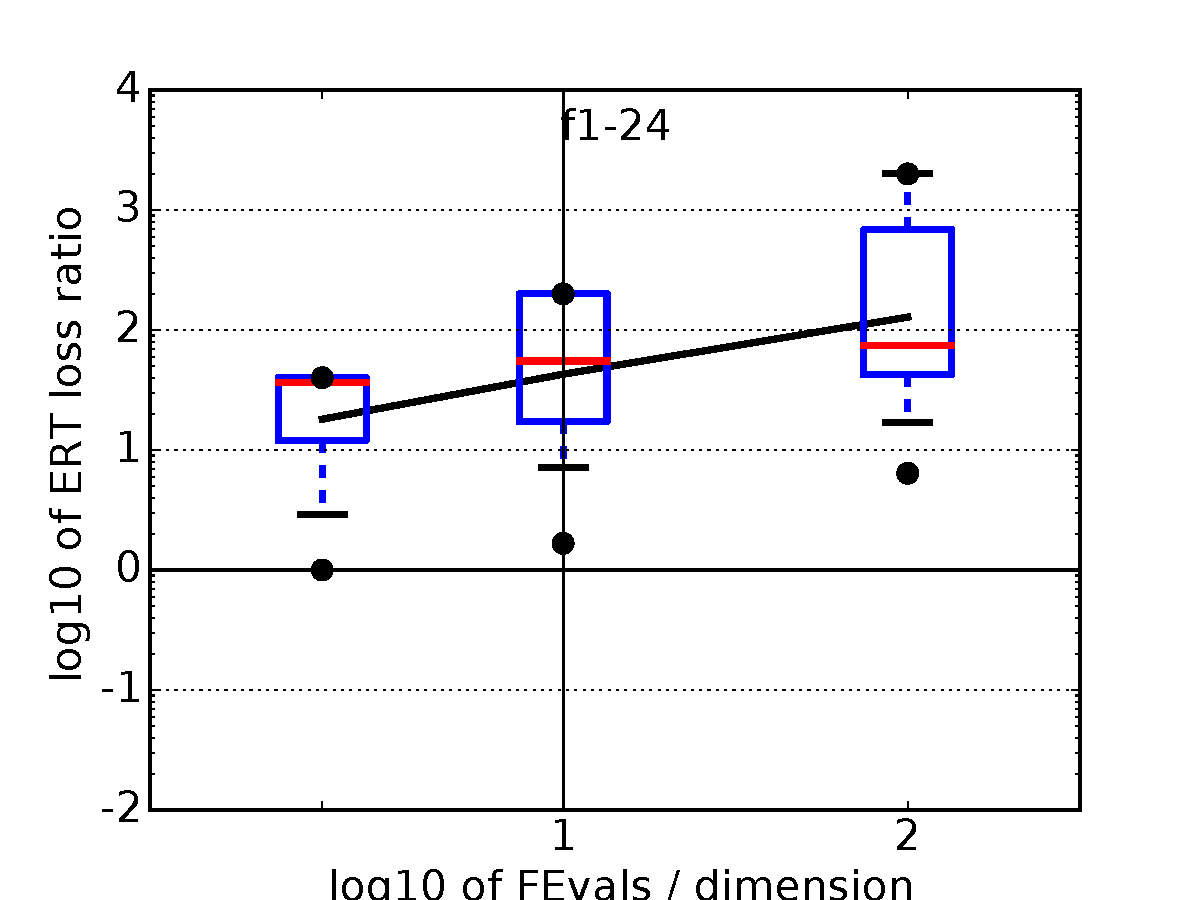
\includegraphics[width=0.24\textwidth,trim=7mm 0 9mm 12mm, clip]{pplogloss_20D_noiselessall}\\[-2ex]
\rot{separable fcts}
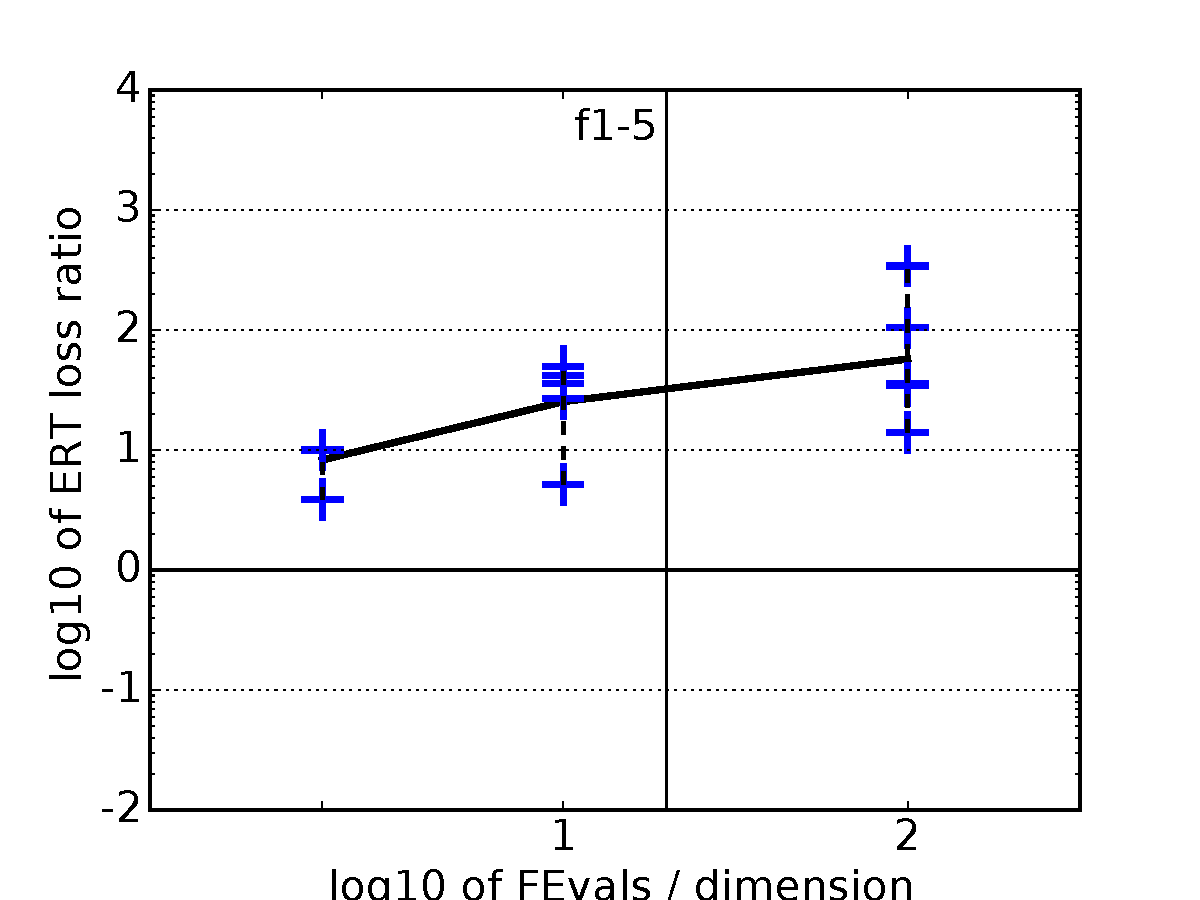
\includegraphics[width=0.35\textwidth,trim=9mm 5mm 18mm 12mm, clip]{pplogloss_05D_separ} &
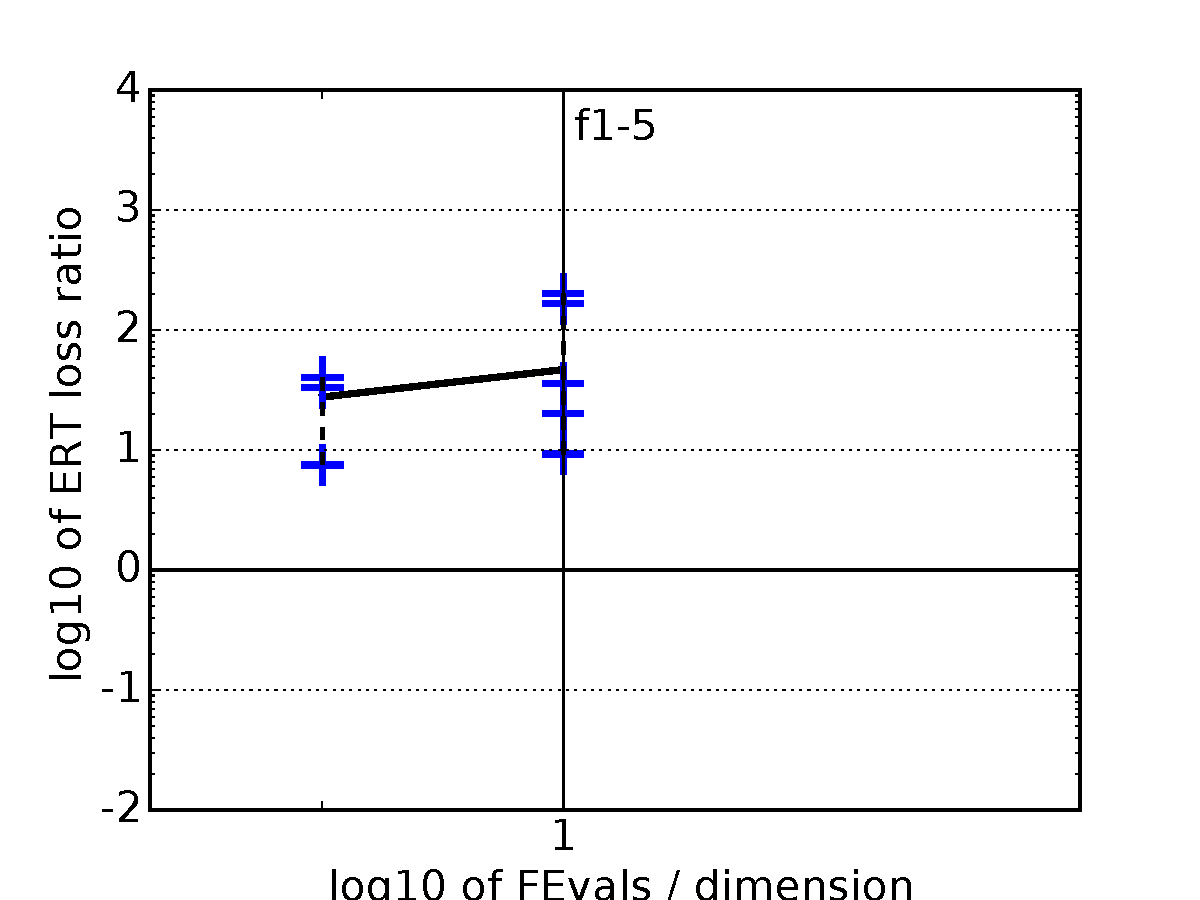
\includegraphics[width=0.35\textwidth,trim=9mm 5mm 18mm 12mm, clip]{pplogloss_20D_separ}\\[-2ex]
\rot[2]{moderate fcts}
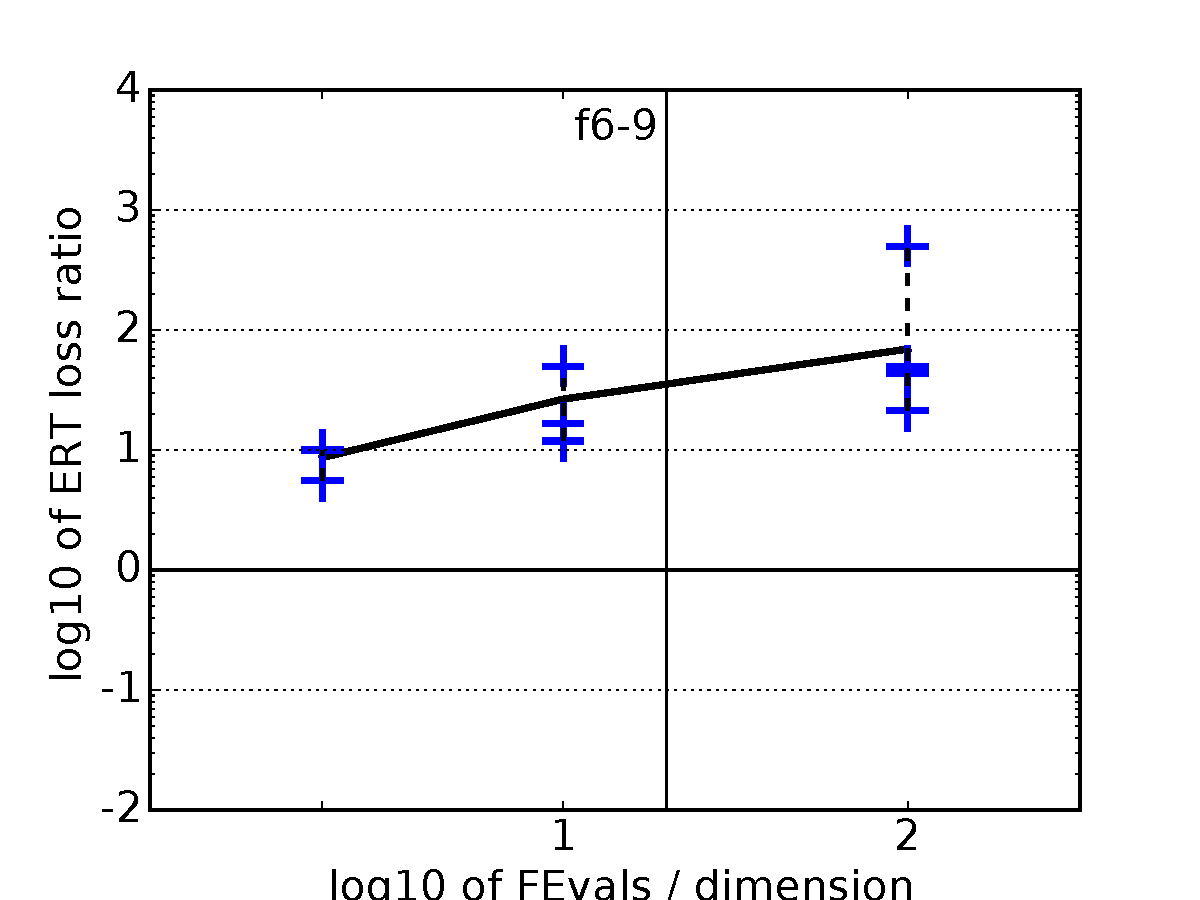
\includegraphics[width=0.35\textwidth,trim=9mm 5mm 18mm 12mm, clip]{pplogloss_05D_lcond} &
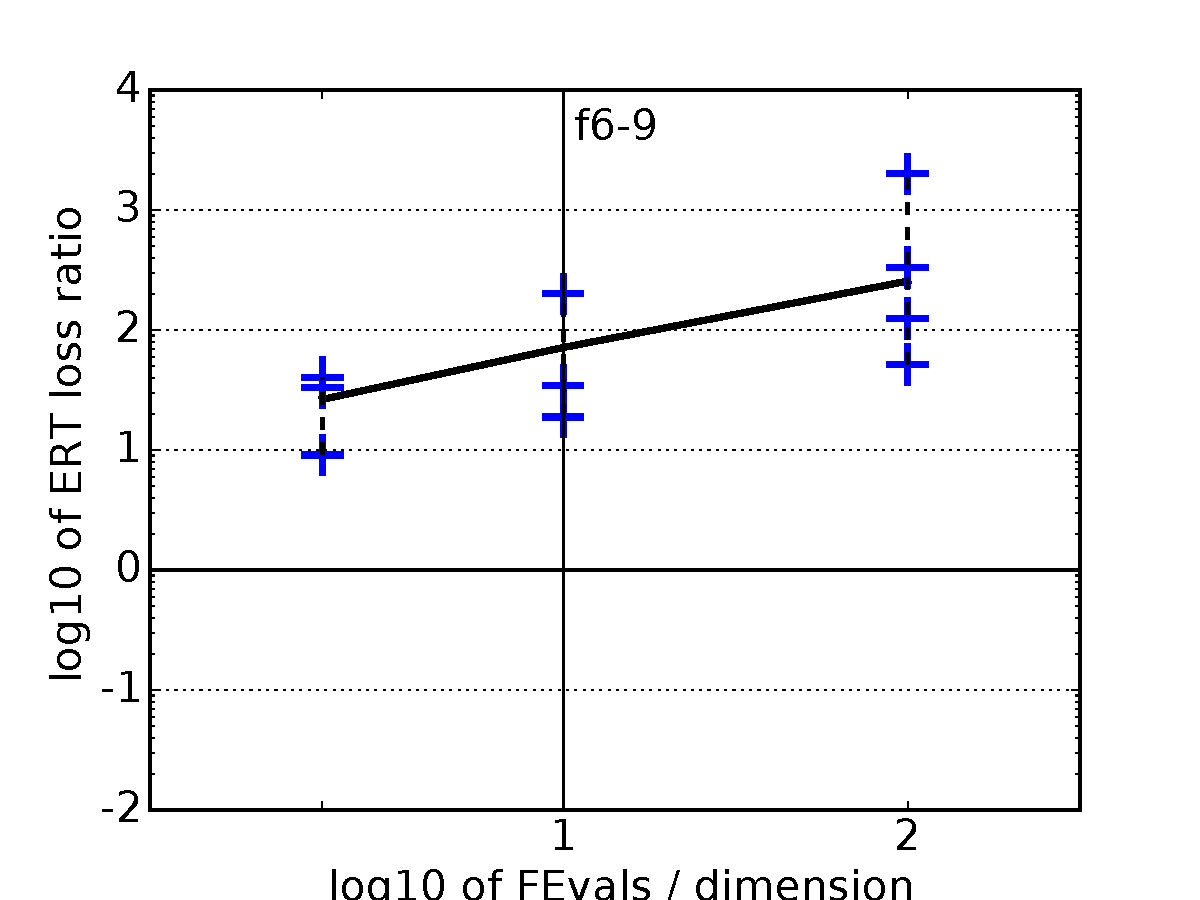
\includegraphics[width=0.35\textwidth,trim=9mm 5mm 18mm 12mm, clip]{pplogloss_20D_lcond}\\[-2ex]
\rot[1.3]{ill-conditioned fcts}
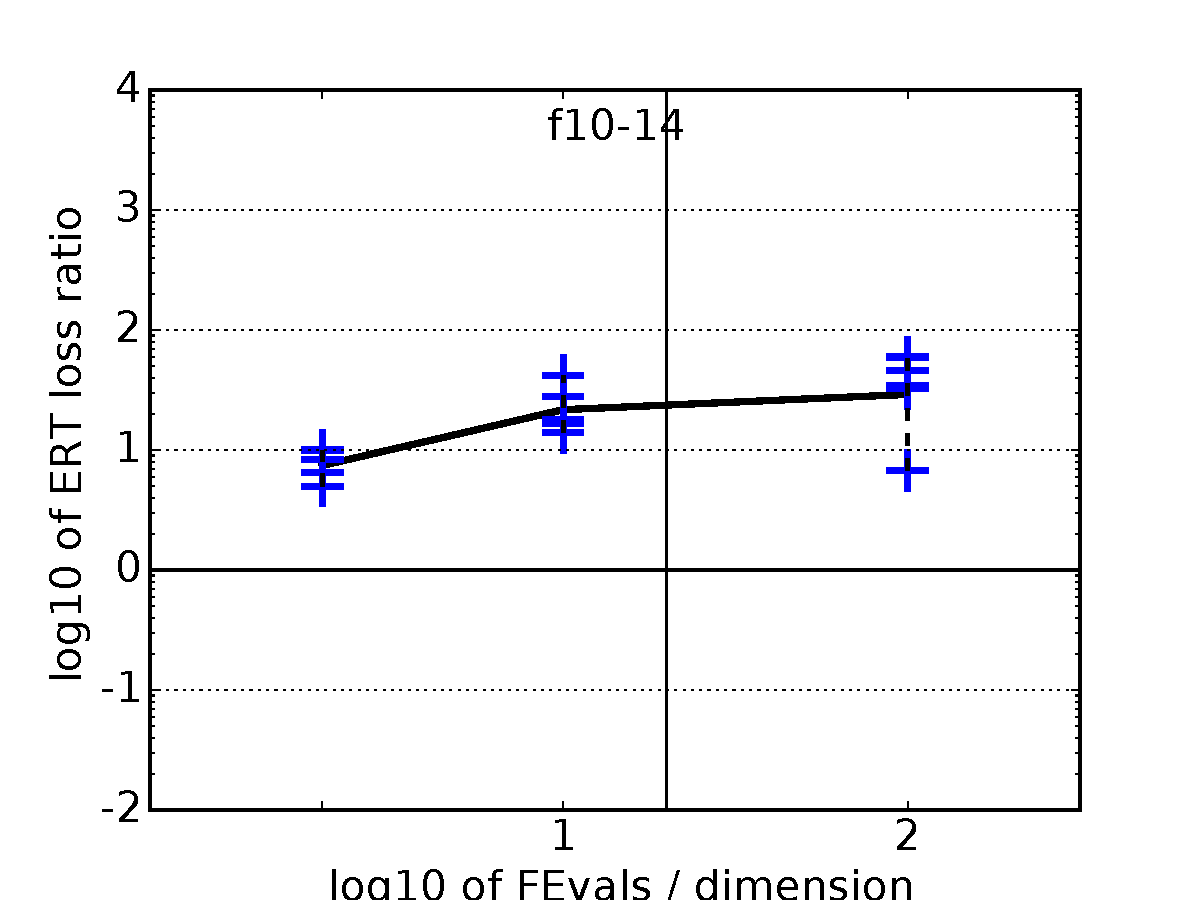
\includegraphics[width=0.35\textwidth,trim=9mm 5mm 18mm 12mm, clip]{pplogloss_05D_hcond} &
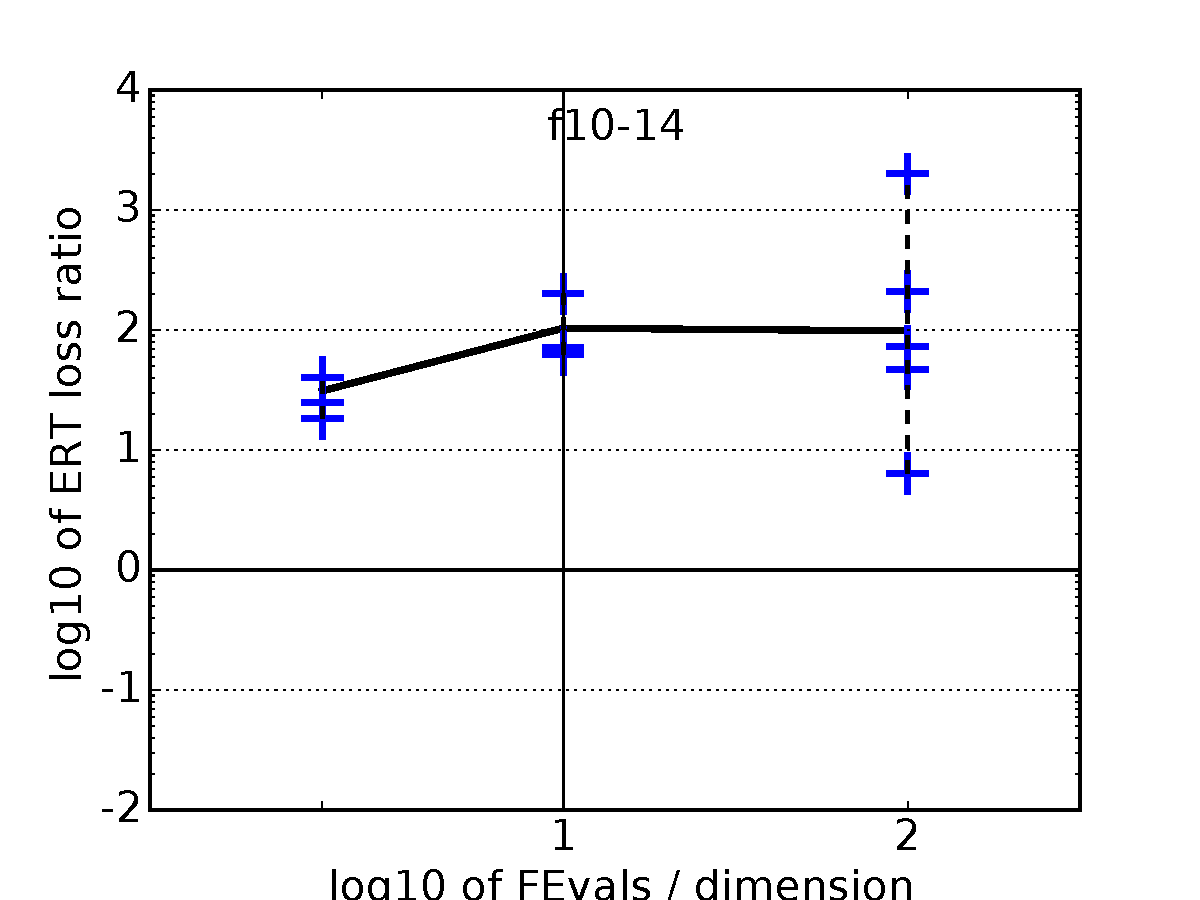
\includegraphics[width=0.35\textwidth,trim=9mm 5mm 18mm 12mm, clip]{pplogloss_20D_hcond}\\[-2ex]
\rot[1.6]{multi-modal fcts}
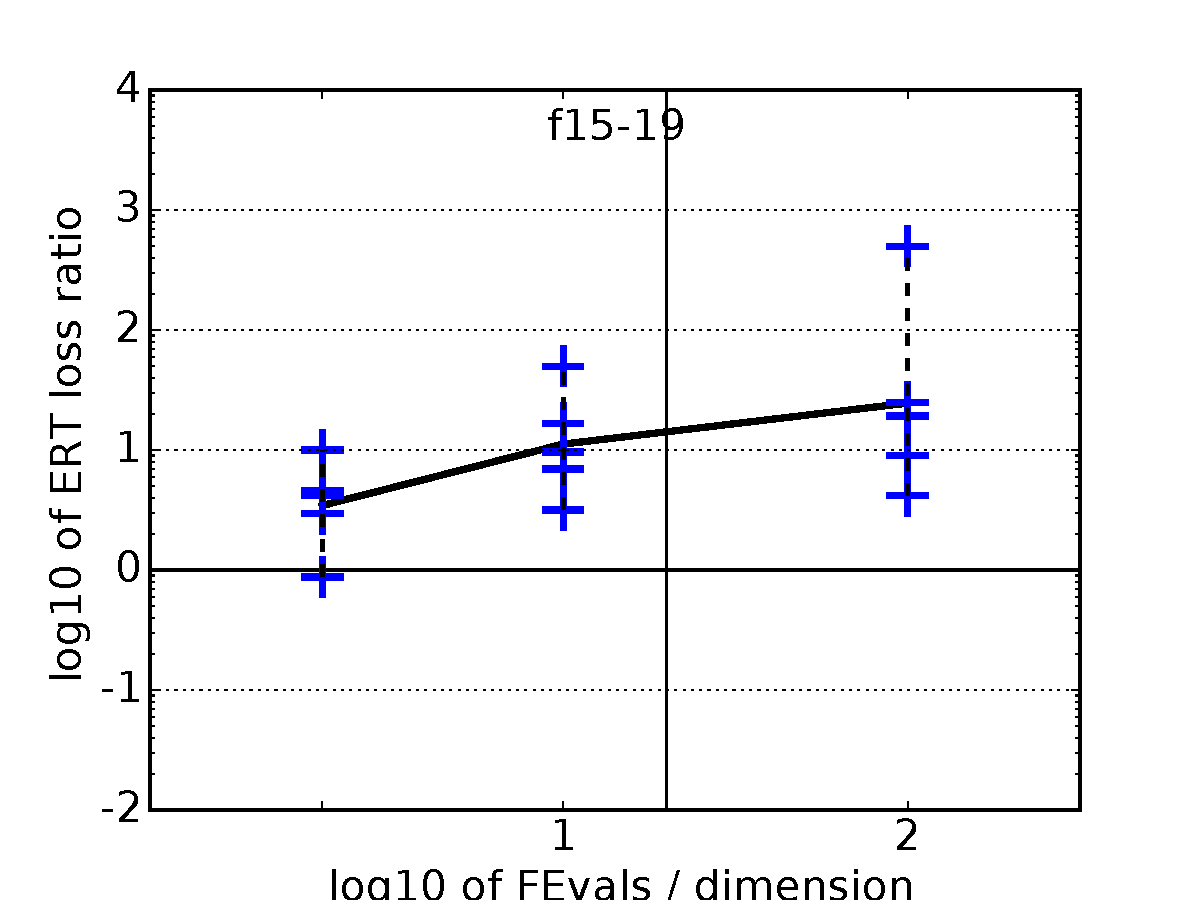
\includegraphics[width=0.35\textwidth,trim=9mm 5mm 18mm 12mm, clip]{pplogloss_05D_multi} &
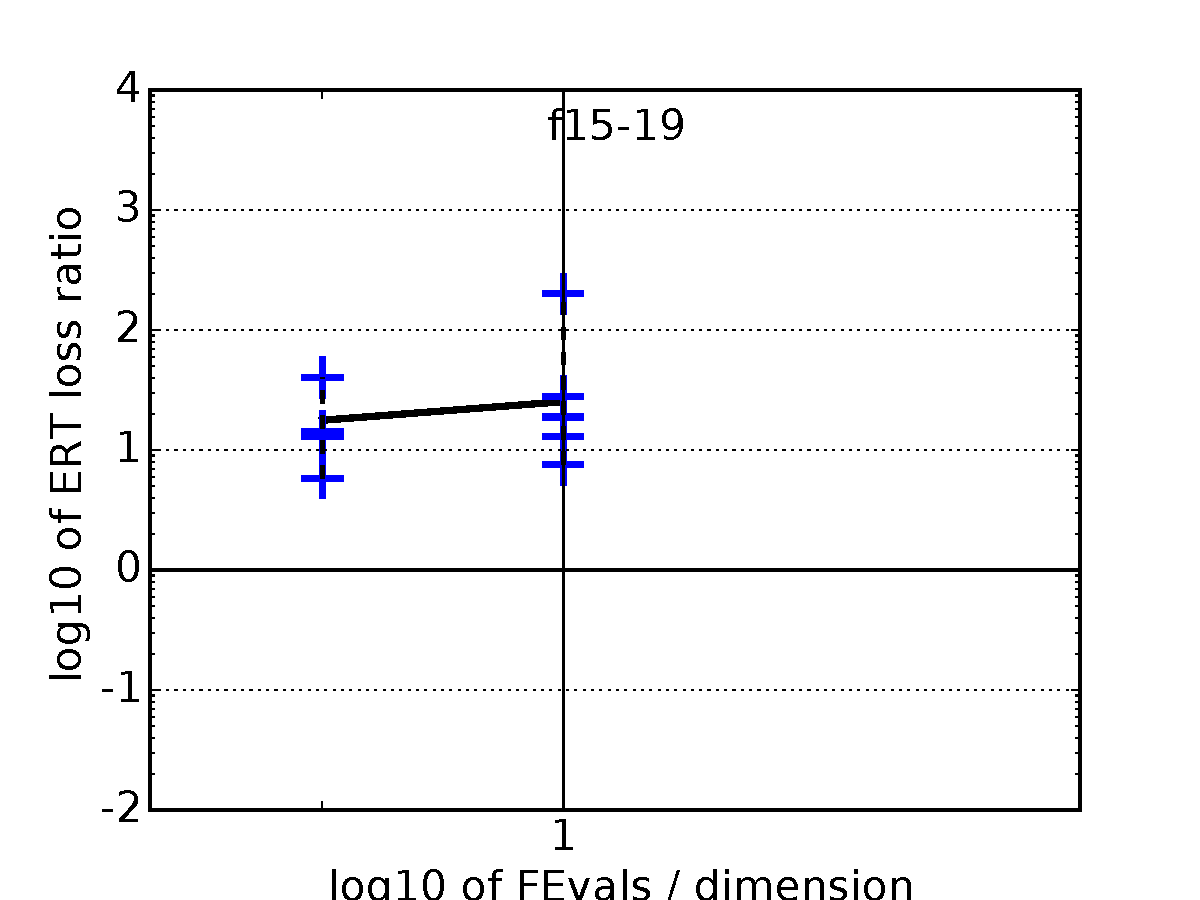
\includegraphics[width=0.35\textwidth,trim=9mm 5mm 18mm 12mm, clip]{pplogloss_20D_multi}\\[-2ex]
\rot[1.0]{weak structure fcts}
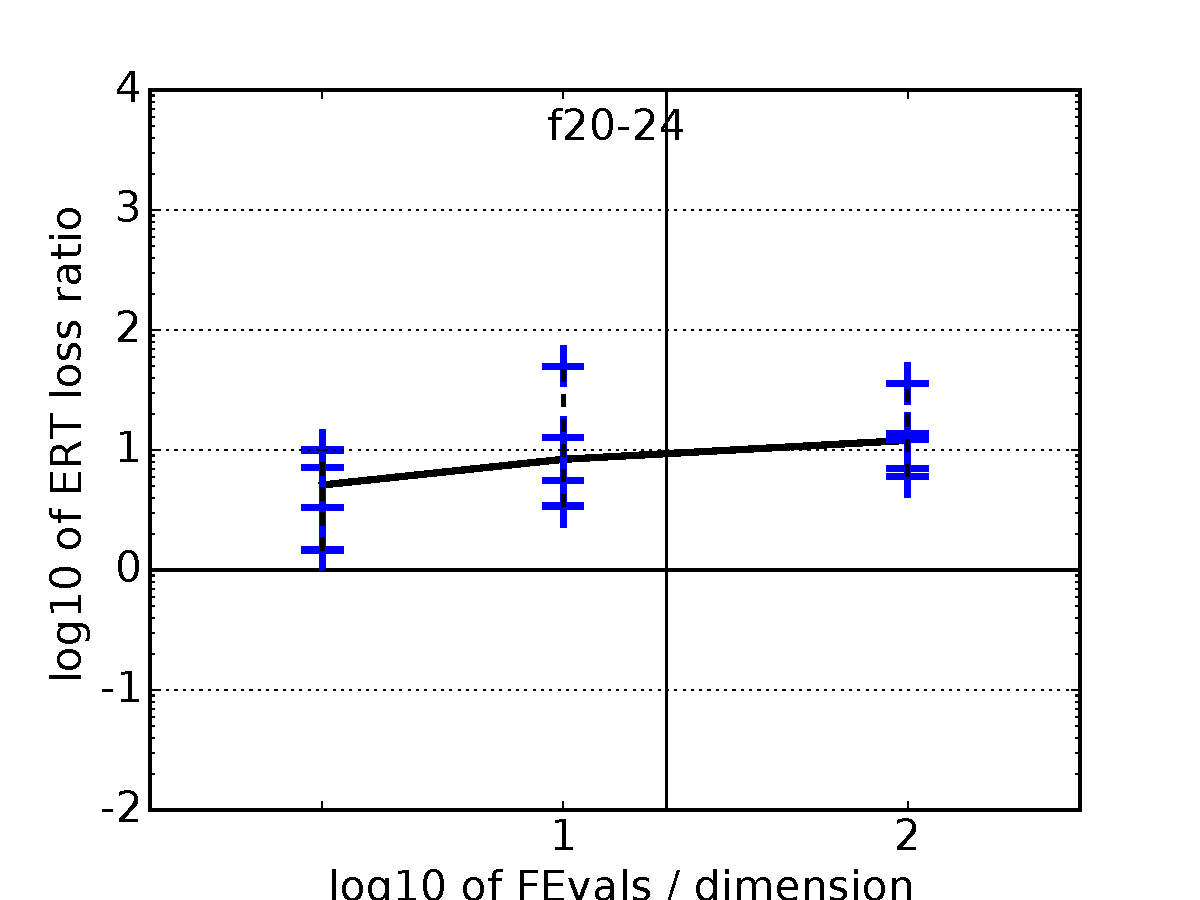
\includegraphics[width=0.35\textwidth,trim=9mm 0mm 18mm 12mm, clip]{pplogloss_05D_mult2} &
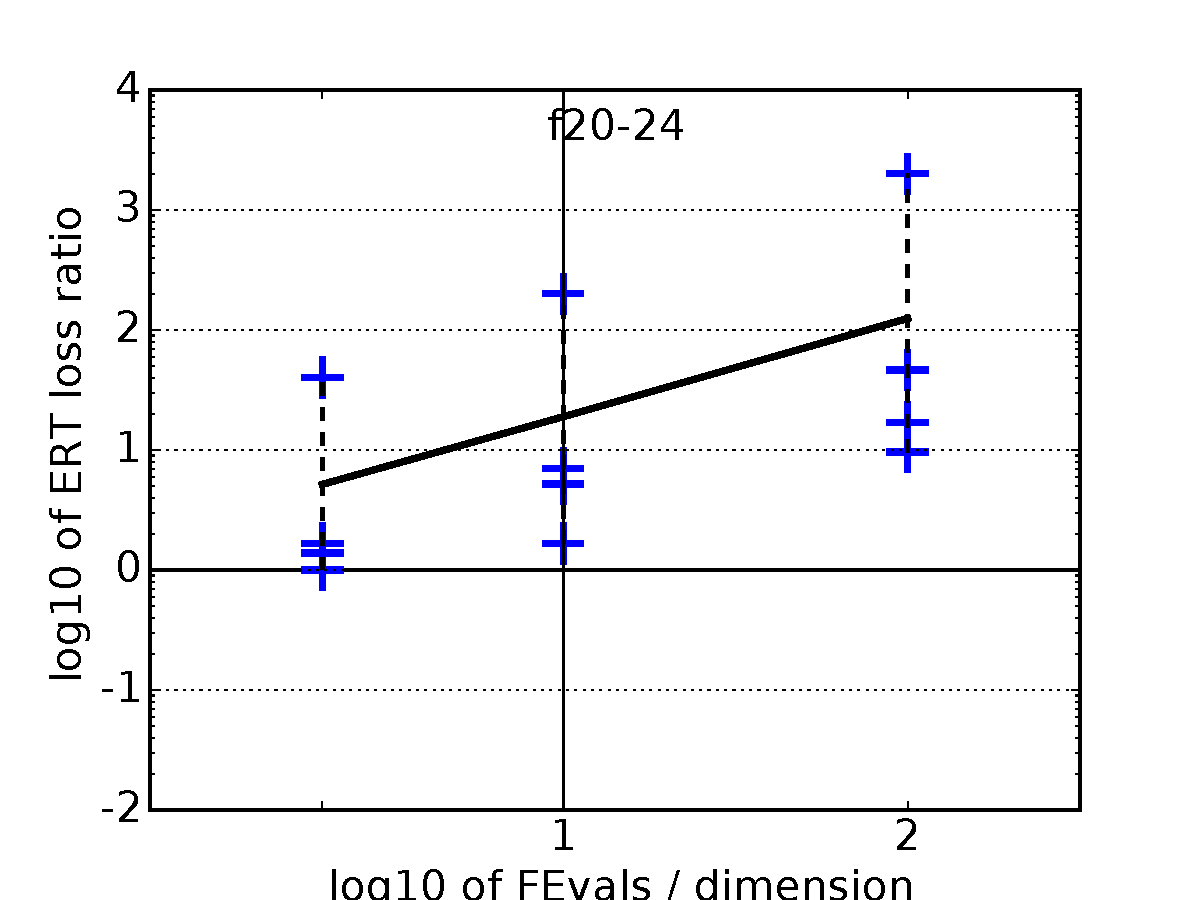
\includegraphics[width=0.35\textwidth,trim=9mm 0mm 18mm 12mm, clip]{pplogloss_20D_mult2}
\vspace*{-1ex}
\end{tabular}
\caption{\label{fig:ERTloglossb\algfolder}\ERT\ loss ratio versus given budget
$\FEvals$ divided by dimension in log-log display. Crosses give
the single values on the indicated functions, the line is the geometric mean.
The vertical line gives the maximal number of function evaluations in the
respective function subgroup.}
\end{figure}
%%%%%%%%%%%%%%%%%%%%%%%%%%%%%%%%%%%%%%%%%%%%%%%%%%%%%%%%%%%%%%%%%%%%%%%%%%%%%%%
%%%%%%%%%%%%%%%%%%%%%%%%%%%%%%%%%%%%%%%%%%%%%%%%%%%%%%%%%%%%%%%%%%%%%%%%%%%%%%%
\begin{figure}[htbp!]
\begin{tabular}{@{}c@{}c@{}c@{}c@{}}
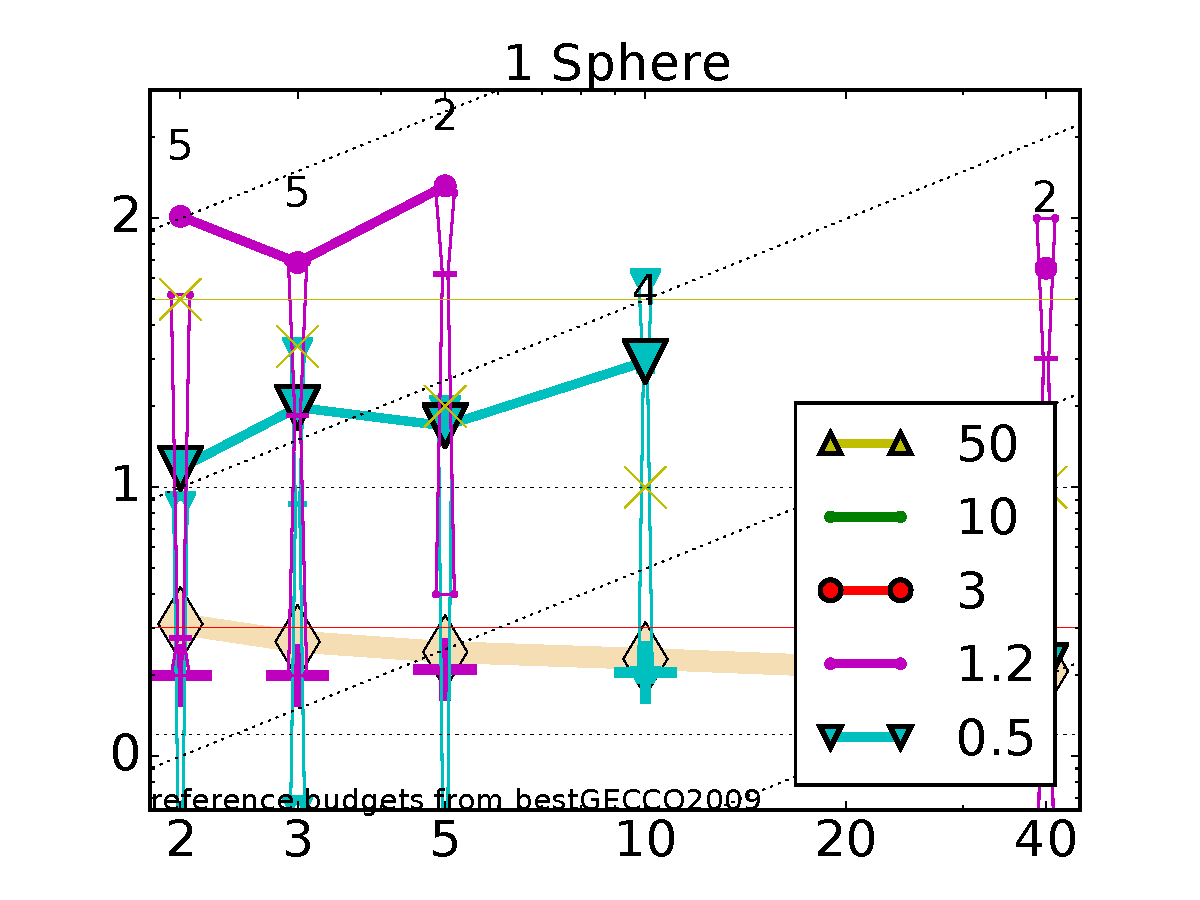
\includegraphics[width=0.25\textwidth, trim=20mm 7mm 15mm 3mm, clip]{ppfigdim_f001}&
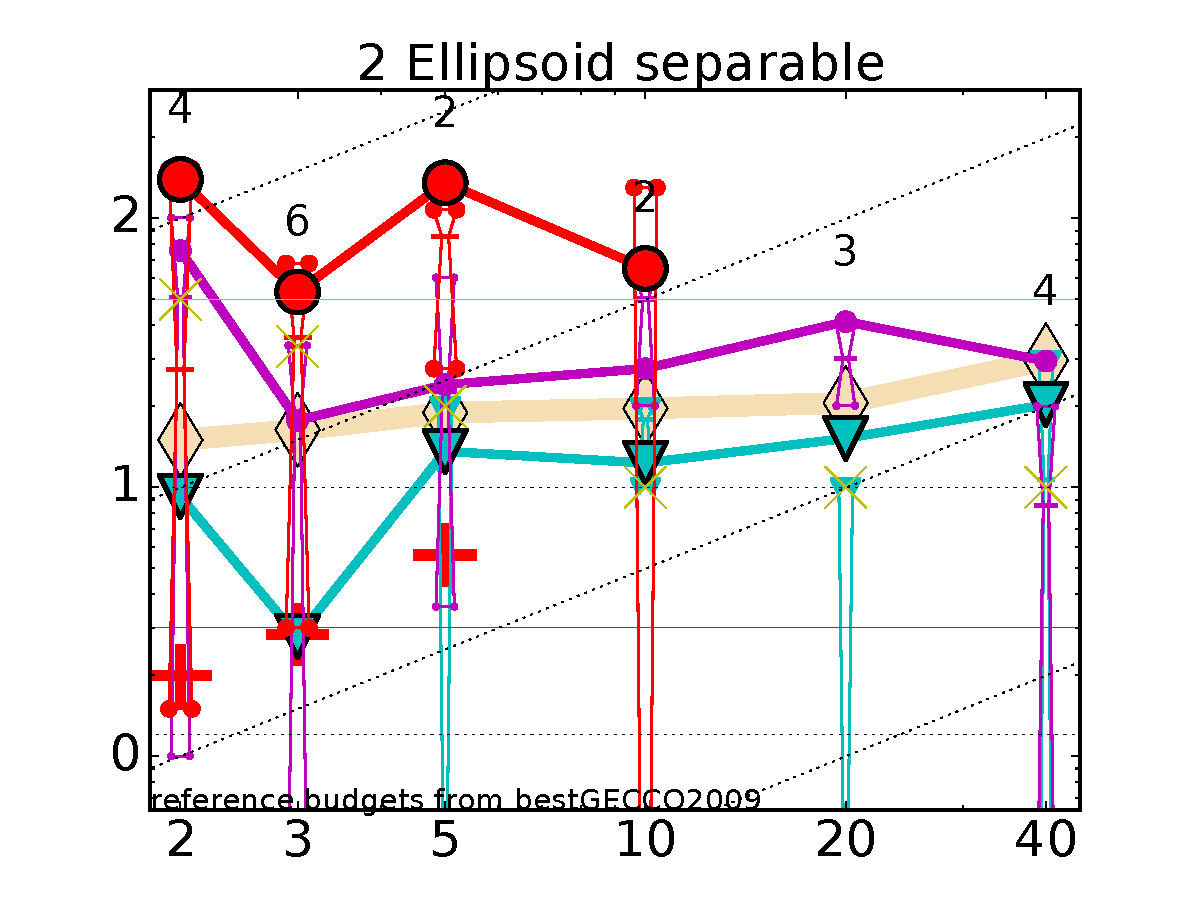
\includegraphics[width=0.25\textwidth, trim=20mm 7mm 15mm 3mm, clip]{ppfigdim_f002}&
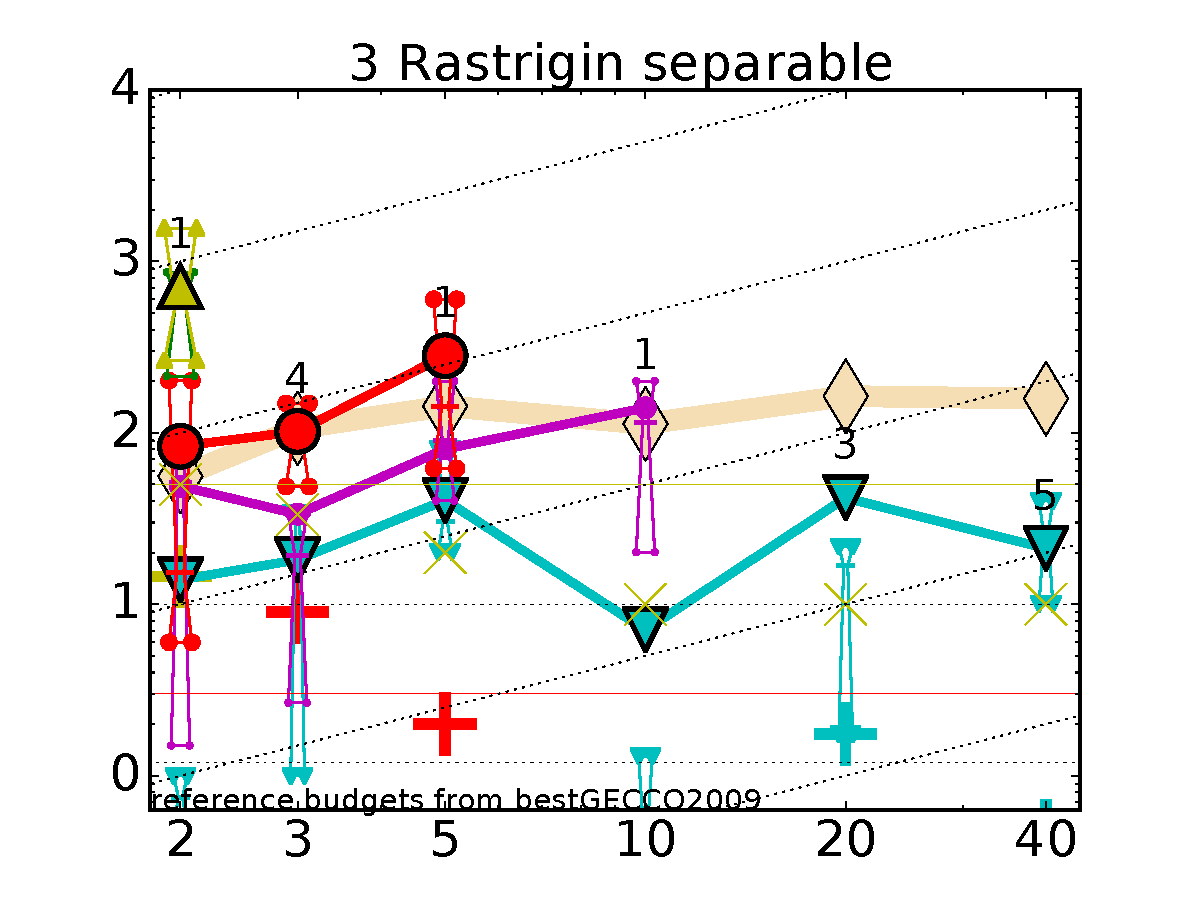
\includegraphics[width=0.25\textwidth, trim=20mm 7mm 15mm 3mm, clip]{ppfigdim_f003}&
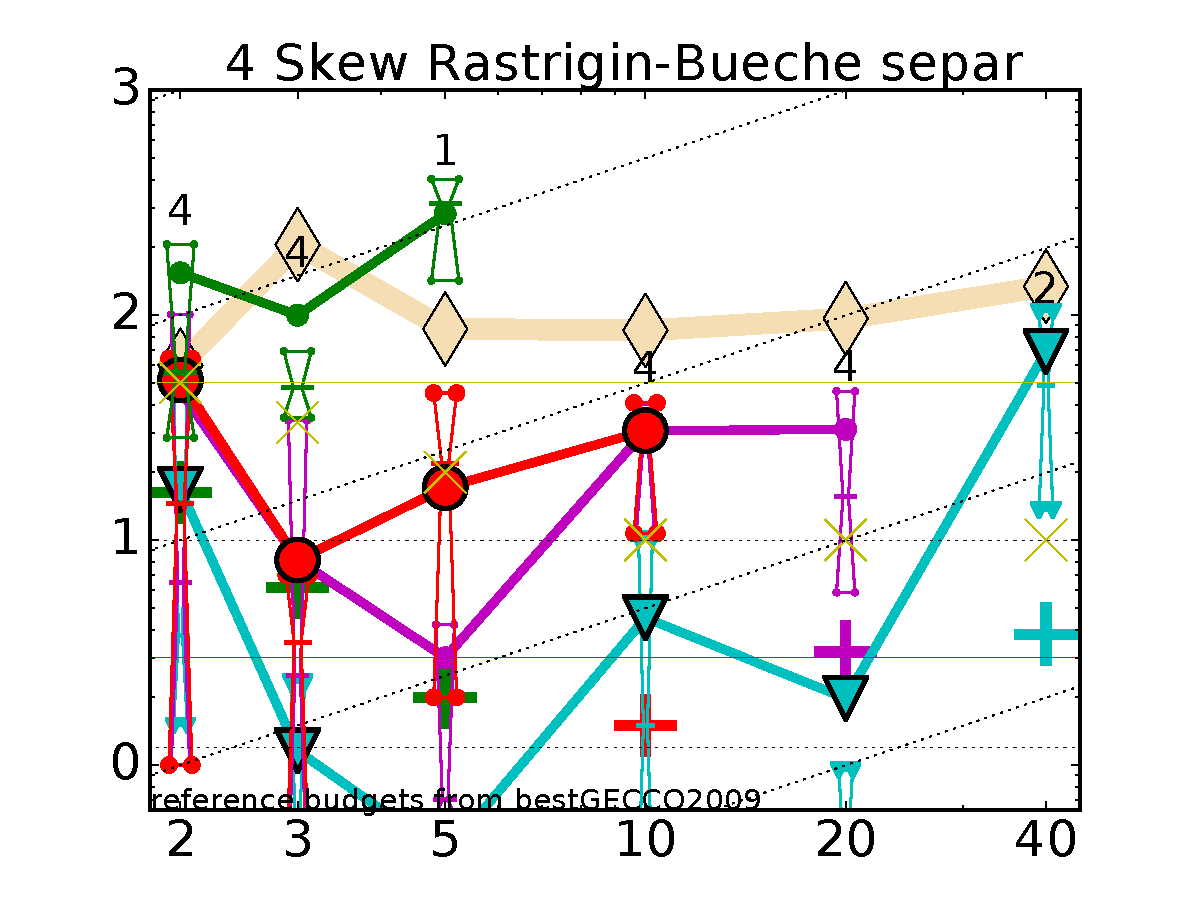
\includegraphics[width=0.25\textwidth, trim=20mm 7mm 15mm 3mm, clip]{ppfigdim_f004}\\
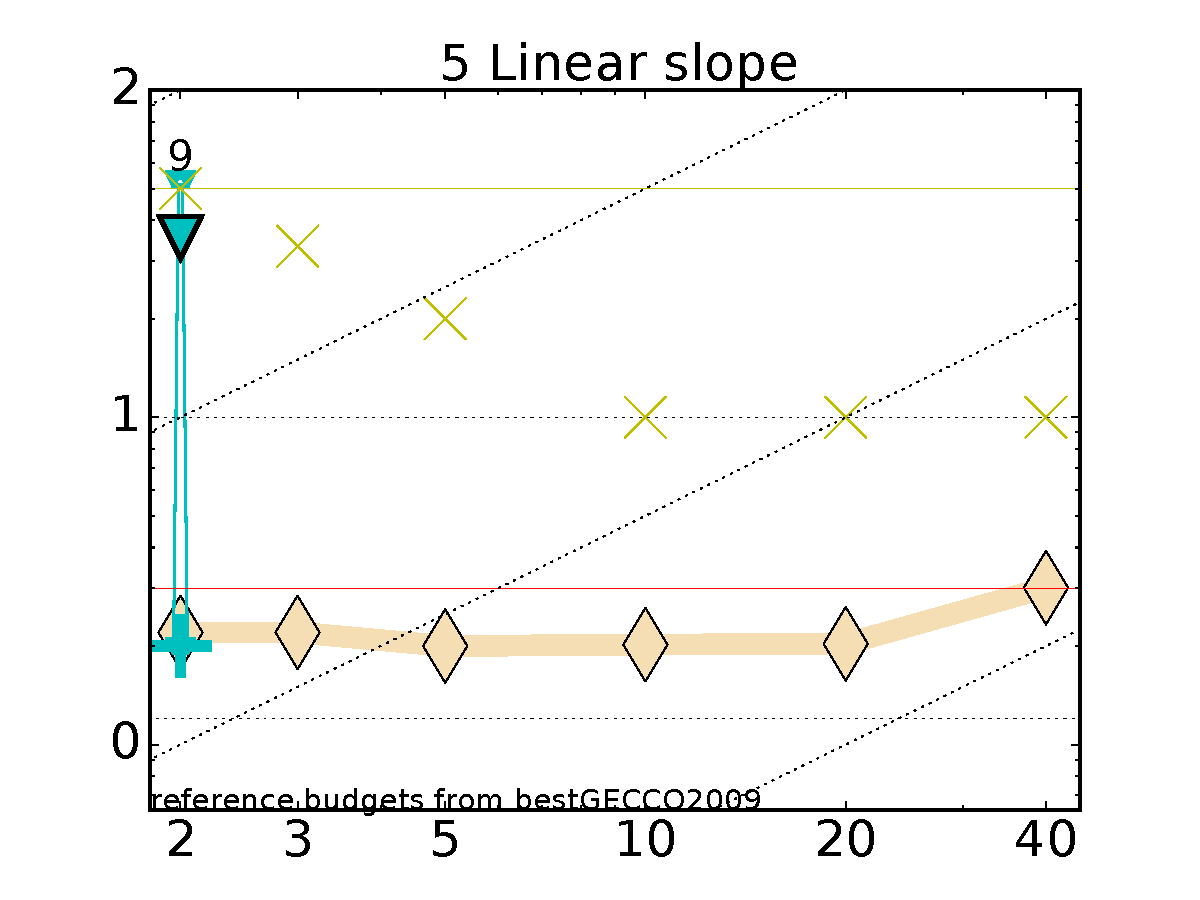
\includegraphics[width=0.25\textwidth, trim=20mm 7mm 15mm 3mm, clip]{ppfigdim_f005}&
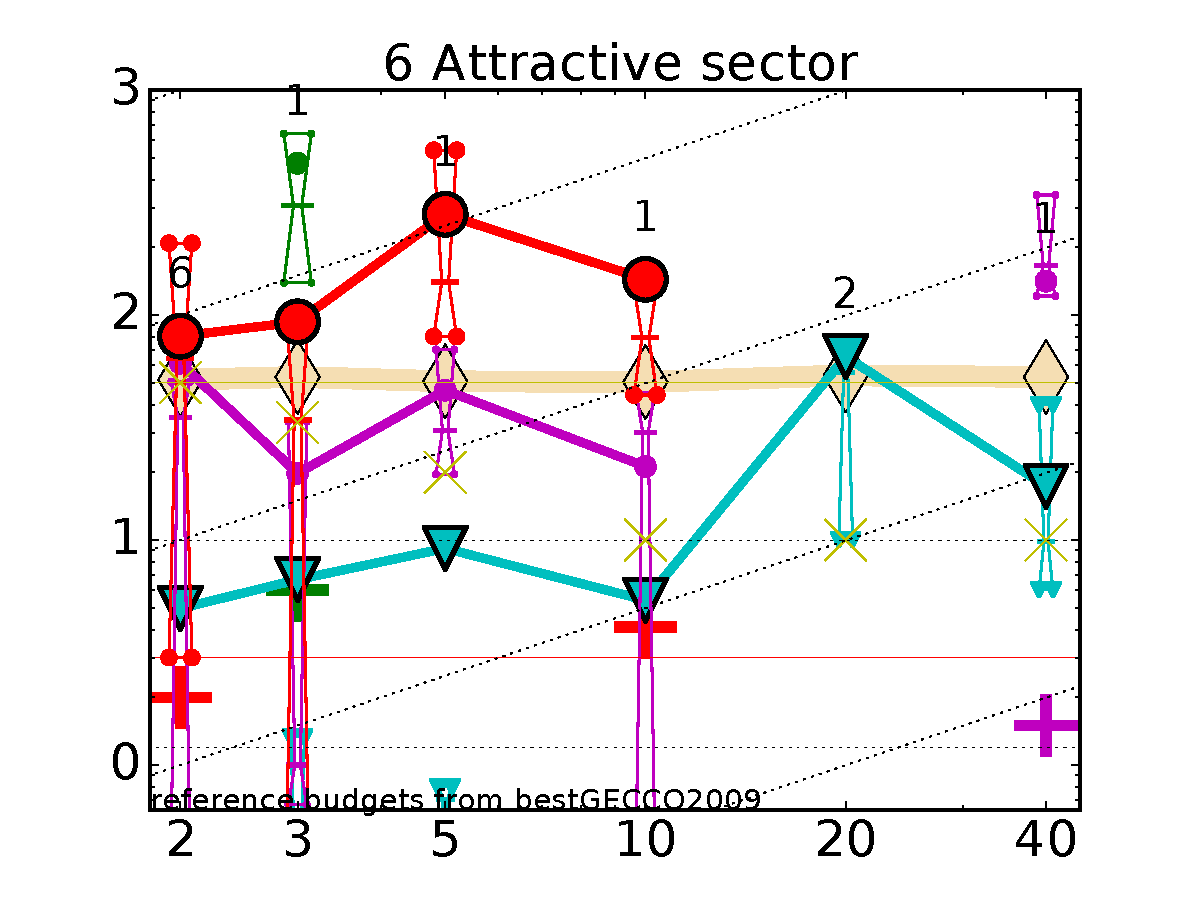
\includegraphics[width=0.25\textwidth, trim=20mm 7mm 15mm 3mm, clip]{ppfigdim_f006}&
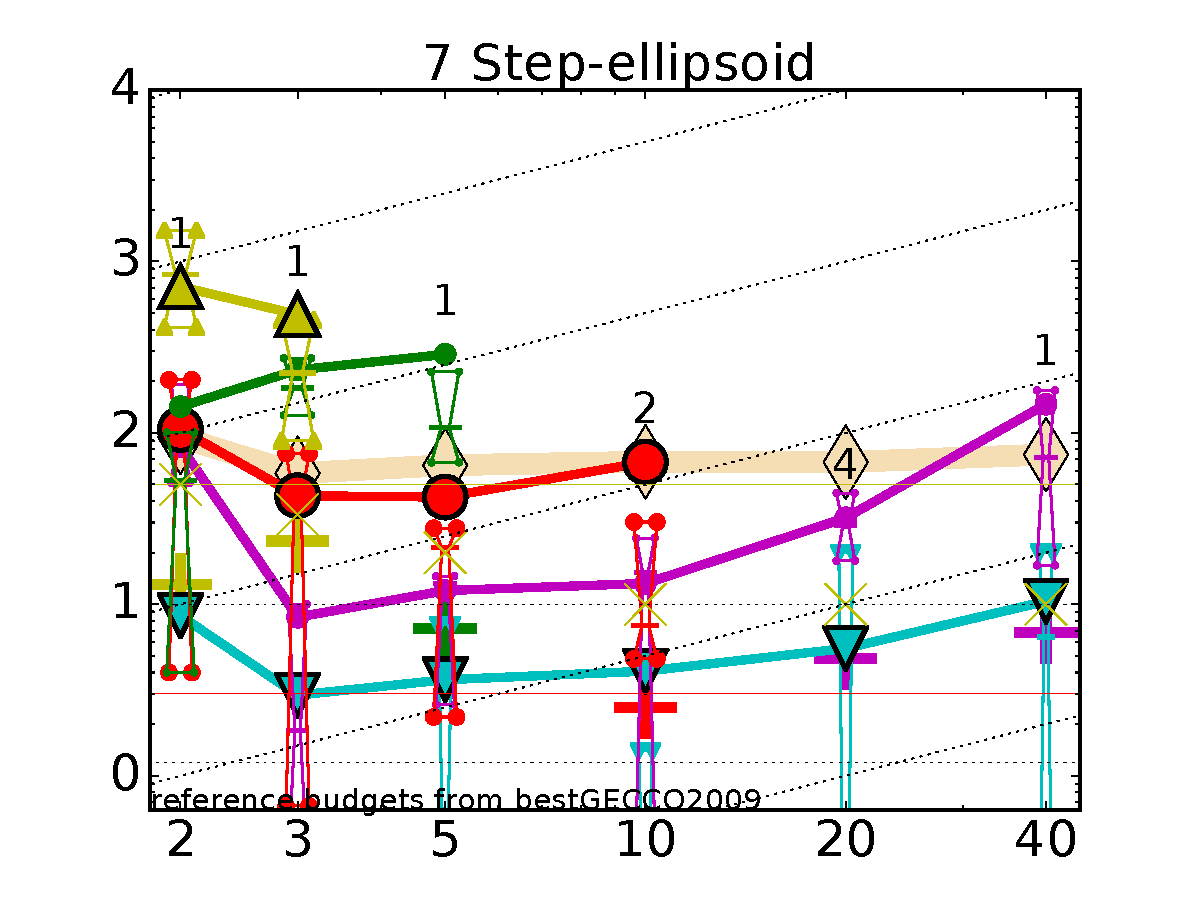
\includegraphics[width=0.25\textwidth, trim=20mm 7mm 15mm 3mm, clip]{ppfigdim_f007}&
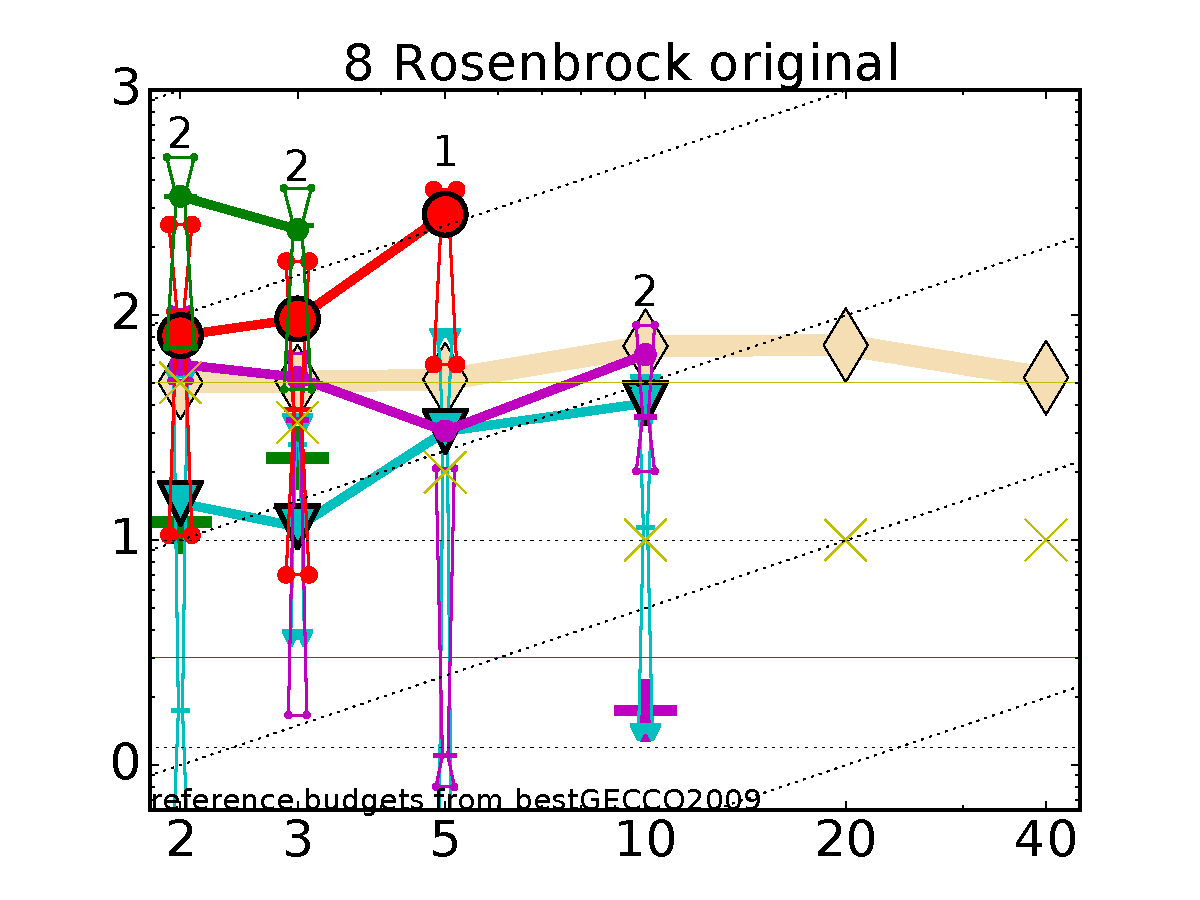
\includegraphics[width=0.25\textwidth, trim=20mm 7mm 15mm 3mm, clip]{ppfigdim_f008}\\
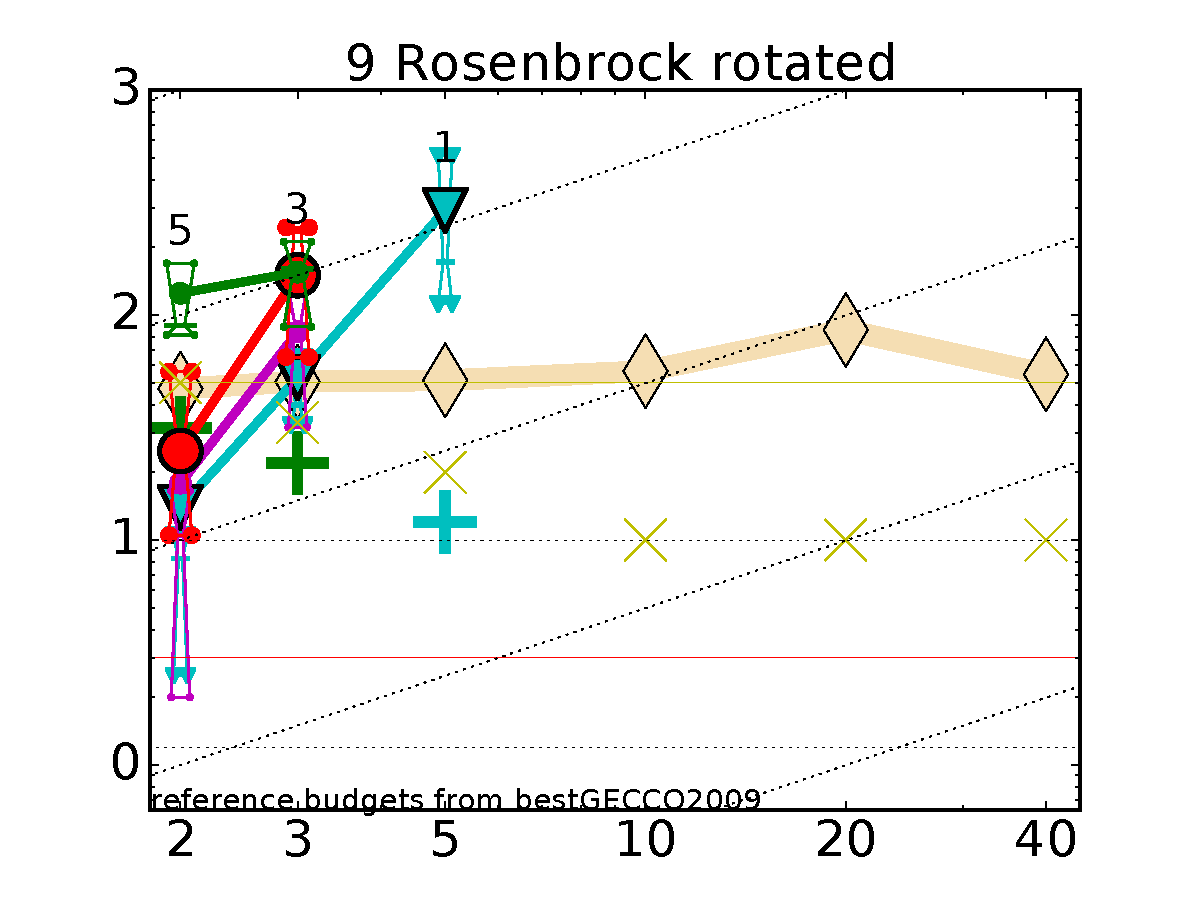
\includegraphics[width=0.25\textwidth, trim=20mm 7mm 15mm 3mm, clip]{ppfigdim_f009}&
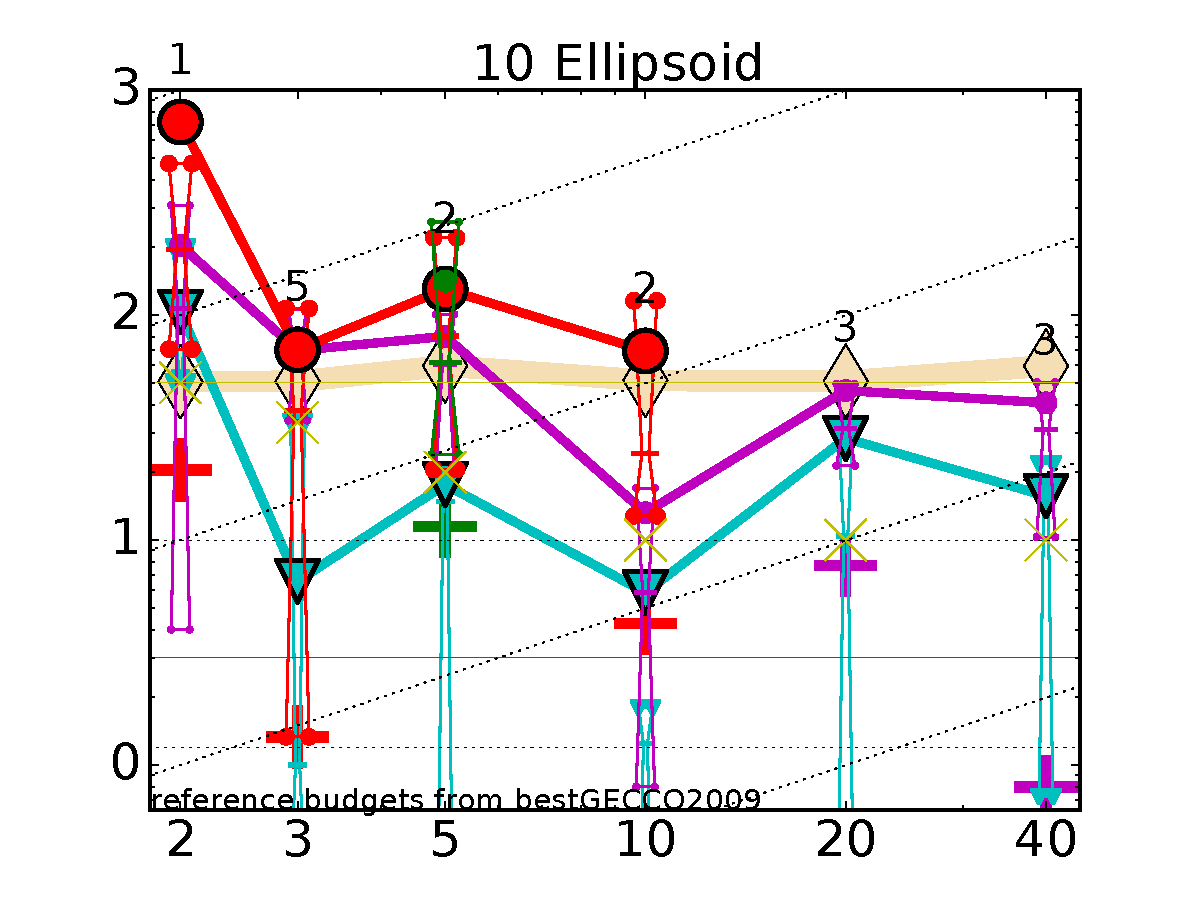
\includegraphics[width=0.25\textwidth, trim=20mm 7mm 15mm 3mm, clip]{ppfigdim_f010}&
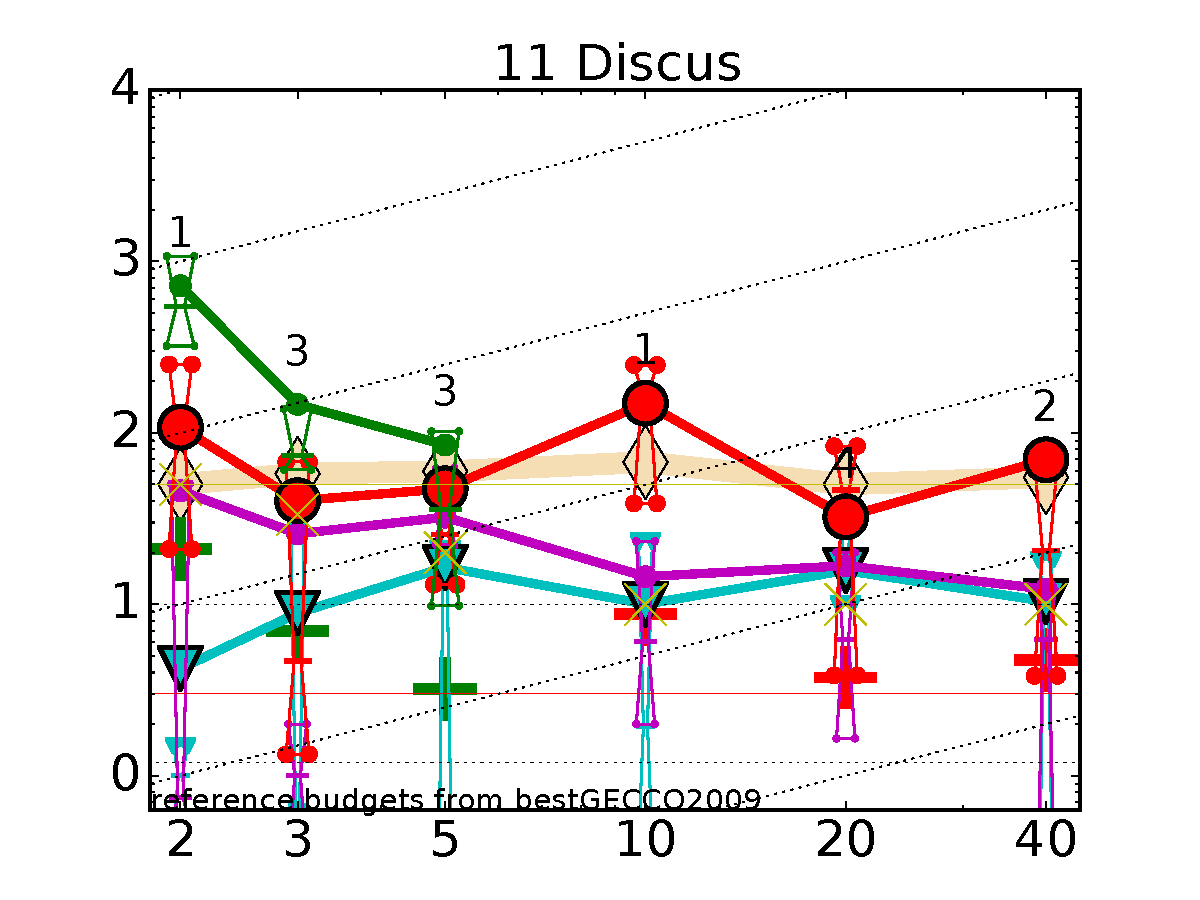
\includegraphics[width=0.25\textwidth, trim=20mm 7mm 15mm 3mm, clip]{ppfigdim_f011}&
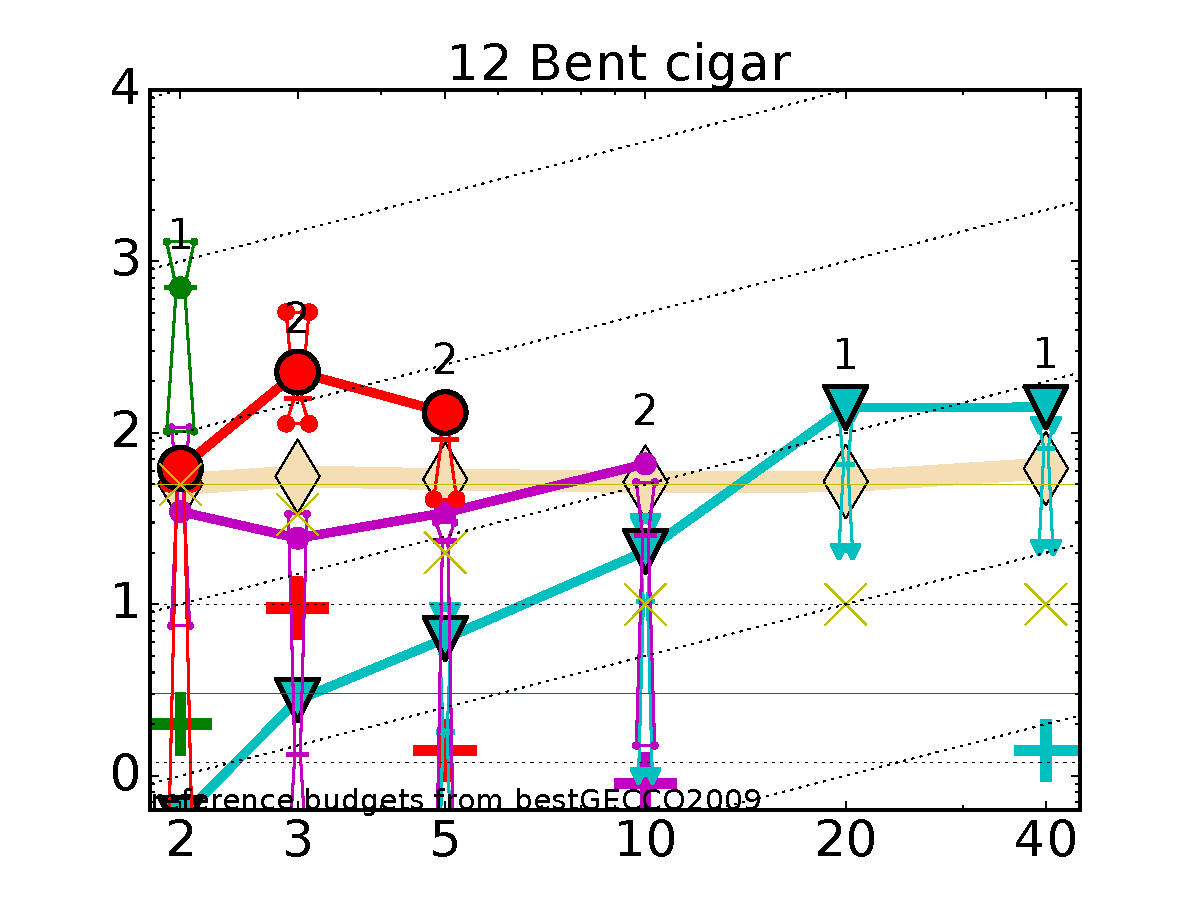
\includegraphics[width=0.25\textwidth, trim=20mm 7mm 15mm 3mm, clip]{ppfigdim_f012}\\
\includegraphics[width=0.25\textwidth, trim=20mm 7mm 15mm 3mm, clip]{ppfigdim_f013}&
\includegraphics[width=0.25\textwidth, trim=20mm 7mm 15mm 3mm, clip]{ppfigdim_f014}&
\includegraphics[width=0.25\textwidth, trim=20mm 7mm 15mm 3mm, clip]{ppfigdim_f015}&
\includegraphics[width=0.25\textwidth, trim=20mm 7mm 15mm 3mm, clip]{ppfigdim_f016}\\
\includegraphics[width=0.25\textwidth, trim=20mm 7mm 15mm 3mm, clip]{ppfigdim_f017}&
\includegraphics[width=0.25\textwidth, trim=20mm 7mm 15mm 3mm, clip]{ppfigdim_f018}&
\includegraphics[width=0.25\textwidth, trim=20mm 7mm 15mm 3mm, clip]{ppfigdim_f019}&
\includegraphics[width=0.25\textwidth, trim=20mm 7mm 15mm 3mm, clip]{ppfigdim_f020}\\
\includegraphics[width=0.25\textwidth, trim=20mm 7mm 15mm 3mm, clip]{ppfigdim_f021}&
\includegraphics[width=0.25\textwidth, trim=20mm 7mm 15mm 3mm, clip]{ppfigdim_f022}&
\includegraphics[width=0.25\textwidth, trim=20mm 7mm 15mm 3mm, clip]{ppfigdim_f023}&
\includegraphics[width=0.25\textwidth, trim=20mm 7mm 15mm 3mm, clip]{ppfigdim_f024}
\end{tabular}
\vspace*{-1ex}
\caption{\label{fig:ERTgraphs\algfolder}
\bbobppfigdimlegend{$f_1$ and $f_{24}$}
%Expected running time (\ERT) divided by
%dimension versus dimension in log-log presentation. Shown are different target
%values $\fopt+\Df$, where 
%% $\Df = 10, 1, 10^{-1}, 10^{-2}, 10^{-3}, 10^{-5}, 10^{-8}$
%$\Df = 10^{\{+1, 0, -1, -2, -3, -5, -8\}}$ and the exponent is given in the
%legend of $f_1$ and $f_{24}$. Plus symbols ($+$) show the median number of
%$f$-evaluations for the best reached target value. Crosses ($\times$) indicate
%the total number of $f$-evaluations ($\nbFEs(-\infty)$) divided by the number
%of trials. Numbers above \ERT-symbols indicate the number of successful trials.
%Y-axis annotations are decimal logarithms.
%%The thick light line with diamond
%%markers shows the single best results from BBOB 2009 for
%%$\Df=10^{-8}$.
}
\end{figure}
%%%%%%%%%%%%%%%%%%%%%%%%%%%%%%%%%%%%%%%%%%%%%%%%%%%%%%%%%%%%%%%%%%%%%%%%%%%%%%%
%%%%%%%%%%%%%%%%%%%%%%%%%%%%%%%%%%%%%%%%%%%%%%%%%%%%%%%%%%%%%%%%%%%%%%%%%%%%%%%
\begin{table}[htbp!]
\centering
\footnotesize
\input{\bbobdatapath\algfolder pptable_05D_noiselessall}
\caption{\label{tab:ERT05D\algfolder} \bbobpptablecaption{} Results of \algname\ in 5-D.}
\end{table}
%%%%%%%%%%%%%%%%%%%%%%%%%%%%%%%%%%%%%%%%%%%%%%%%%%%%%%%%%%%%%%%%%%%%%%%%%%%%%%%
%%%%%%%%%%%%%%%%%%%%%%%%%%%%%%%%%%%%%%%%%%%%%%%%%%%%%%%%%%%%%%%%%%%%%%%%%%%%%%%
\begin{table}[htbp!]
\centering
\footnotesize
\input{\bbobdatapath\algfolder pptable_20D_noiselessall}
\caption{\label{tab:ERT20D\algfolder} \bbobpptablecaption{} Results of \algname\ in 20-D.}
\end{table}
%%%%%%%%%%%%%%%%%%%%%%%%%%%%%%%%%%%%%%%%%%%%%%%%%%%%%%%%%%%%%%%%%%%%%%%%%%%%%%%
%%%%%%%%%%%%%%%%%%%%%%%%%%%%%%%%%%%%%%%%%%%%%%%%%%%%%%%%%%%%%%%%%%%%%%%%%%%%%%%
% The following two commands are all you need in the
% initial runs of your .tex file to
% produce the bibliography for the citations in your paper.
\bibliographystyle{abbrv}
\bibliography{bbob} % bbob.bib is the name of the bib file in this case
% You must have a proper ".bib" file
%  and remember to run:
% latex bibtex latex latex
% to resolve all references
\end{document}

